%Version 3.1 December 2024
% See section 11 of the User Manual for version history
%
%%%%%%%%%%%%%%%%%%%%%%%%%%%%%%%%%%%%%%%%%%%%%%%%%%%%%%%%%%%%%%%%%%%%%%
%%                                                                 %%
%% Please do not use \input{...} to include other tex files.       %%
%% Submit your LaTeX manuscript as one .tex document.              %%
%%                                                                 %%
%% All additional figures and files should be attached             %%
%% separately and not embedded in the \TeX\ document itself.       %%
%%                                                                 %%
%%%%%%%%%%%%%%%%%%%%%%%%%%%%%%%%%%%%%%%%%%%%%%%%%%%%%%%%%%%%%%%%%%%%%

%%\documentclass[referee,sn-basic]{sn-jnl}% referee option is meant for double line spacing

%%=======================================================%%
%% to print line numbers in the margin use lineno option %%
%%=======================================================%%

%%\documentclass[lineno,pdflatex,sn-basic]{sn-jnl}% Basic Springer Nature Reference Style/Chemistry Reference Style

%%=========================================================================================%%
%% the documentclass is set to pdflatex as default. You can delete it if not appropriate.  %%
%%=========================================================================================%%

%%\documentclass[sn-basic]{sn-jnl}% Basic Springer Nature Reference Style/Chemistry Reference Style

%%Note: the following reference styles support Namedate and Numbered referencing. By default the style follows the most common style. To switch between the options you can add or remove “Numbered” in the optional parenthesis. 
%%The option is available for: sn-basic.bst, sn-chicago.bst%  
 
%%\documentclass[pdflatex,sn-nature]{sn-jnl}% Style for submissions to Nature Portfolio journals
%%\documentclass[pdflatex,sn-basic]{sn-jnl}% Basic Springer Nature Reference Style/Chemistry Reference Style
%%\documentclass[iicol, pdflatex,sn-mathphys-num]{sn-jnl}% Math and Physical Sciences Numbered Reference Style
%%\documentclass[pdflatex,sn-mathphys-ay]{sn-jnl}% Math and Physical Sciences Author Year Reference Style
\documentclass[pdflatex,sn-mathphys-num]{sn-jnl}
\usepackage[T1]{fontenc}
%%\documentclass[pdflatex,sn-aps]{sn-jnl}% American Physical Society (APS) Reference Style
%%\documentclass[pdflatex,sn-vancouver-num]{sn-jnl}% Vancouver Numbered Reference Style
%%\documentclass[pdflatex,sn-vancouver-ay]{sn-jnl}% Vancouver Author Year Reference Style
%%\documentclass[pdflatex,sn-apa]{sn-jnl}% APA Reference Style
%%\documentclass[pdflatex,sn-chicago]{sn-jnl}% Chicago-based Humanities Reference Style

%%%% Standard Packages
%%<additional latex packages if required can be included here>

\usepackage{mathrsfs}%
\usepackage{graphicx}%
\usepackage{multirow}%
\usepackage{amsmath,amssymb,amsfonts}%
\usepackage{amsthm}%
\usepackage[title]{appendix}%
\usepackage{xcolor}%
\usepackage{textcomp}%
\usepackage{manyfoot}%
\usepackage{booktabs}%
\usepackage{algorithm}%
\usepackage{algorithmicx}%
\usepackage{algpseudocode}%
\usepackage{listings}%
\usepackage[normalem]{ulem}
\usepackage{caption}
\usepackage{subcaption}
\usepackage{soul}
%%%%

%%%%%=============================================================================%%%%
%%%%  Remarks: This template is provided to aid authors with the preparation
%%%%  of original research articles intended for submission to journals published 
%%%%  by Springer Nature. The guidance has been prepared in partnership with 
%%%%  production teams to conform to Springer Nature technical requirements. 
%%%%  Editorial and presentation requirements differ among journal portfolios and 
%%%%  research disciplines. You may find sections in this template are irrelevant 
%%%%  to your work and are empowered to omit any such section if allowed by the 
%%%%  journal you intend to submit to. The submission guidelines and policies 
%%%%  of the journal take precedence. A detailed User Manual is available in the 
%%%%  template package for technical guidance.
%%%%%=============================================================================%%%%

%% as per the requirement new theorem styles can be included as shown below
\theoremstyle{thmstyleone}%
\newtheorem{theorem}{Theorem}%  meant for continuous numbers
%%\newtheorem{theorem}{Theorem}[section]% meant for sectionwise numbers
%% optional argument [theorem] produces theorem numbering sequence instead of independent numbers for Proposition
\newtheorem{proposition}[theorem]{Proposition}% 
%%\newtheorem{proposition}{Proposition}% to get separate numbers for theorem and proposition etc.

\theoremstyle{thmstyletwo}%
\newtheorem{example}{Example}%
\newtheorem{remark}{Remark}%

\theoremstyle{thmstylethree}%
\newtheorem{definition}{Definition}%

\raggedbottom
%%\unnumbered% uncomment this for unnumbered level heads

\begin{document}

\title[Article Title]{A Comparative Study of Mobile Robot Localization Methods in Indoor–Outdoor Transition Scenarios}


%%=============================================================%%
%% Prefix	-> \pfx{Dr}
%% GivenName	-> \fnm{Joergen W.}
%% Particle	-> \spfx{van der} -> surname prefix
%% FamilyName	-> \sur{Ploeg}
%% Suffix	-> \sfx{IV}
%% NatureName	-> \tanm{Poet Laureate} -> Title after name
%% Degrees	-> \dgr{MSc, PhD}
%% \author*[1,2]{\pfx{Dr} \fnm{Joergen W.} \spfx{van der} \sur{Ploeg} \sfx{IV} \tanm{Poet Laureate} 
%%                 \dgr{MSc, PhD}}\email{iauthor@gmail.com}
%%=============================================================%%


\author[1, 2]{\fnm{Katarzyna} \sur{Kijania}}\email{katarzyna.kijania@dokt.pw.edu.pl}
% ORCID: 0000-0003-3824-9525

\author[1]{\fnm{Jacek} \sur{Dybała}}\email{jacek.dybala@pw.edu.pl}
% ORCID: 0000-0002-0721-1105

\author*[3]{\fnm{Piotr} \sur{Duszak}}\email{piotr.duszak@pw.edu.pl} 
% ORCID: 0000-0001-6059-702X


\affil[1]{\orgname{Warsaw University of Technology}, \orgdiv{Faculty of Automotive and Construction Machinery Engineering}, \orgaddress{\street{Ludwika Narbutta 84}, \postcode{02-524} \city{Warsaw}, \country{Poland}}}


\affil[2]{\orgname{Łukasiewicz Research Network - Automotive Industry Institute (Łukasiewicz-PIMOT)}, \orgaddress{\street{Jagiellońska 55}, \postcode{03-301} \city{Warsaw}, \country{Poland}}}

\affil[3]{\orgname{Warsaw University of Technology}, \orgdiv{Faculty of Mechatronics}, \orgaddress{\street{Andrzeja Boboli 8}, \postcode{02-525} \city{Warsaw}, \country{Poland}}}

\abstract{
Reliable localization across indoor–outdoor transitions remains a major challenge for autonomous mobile robots due to abrupt changes in environmental geometry and illumination that can severely degrade localization accuracy. This paper investigates the phenomenon referred to as a stability shock, defined as a~sudden increase in localization uncertainty and estimation error during physical transitions between indoor and outdoor environments. We present a~comprehensive evaluation of six state-of-the-art localization algorithms—FAST-LIO2, GLIM, KISS-ICP, ORB-SLAM3, RKO-LIO, and TSformer-VO—using the high-precision Oxford Spires dataset. To enable transition-specific performance analysis, we \hl{apply a reproducible, timestamp-based trajectory segmentation} method that partitions robot trajectories into indoor, outdoor, and transition segments. This methodology isolates localization errors associated with environmental transitions, which are typically obscured in conventional full-trajectory evaluations, and enables a~quantitative assessment of their impact on localization performance. Experimental results show that localization methods based on 3D LiDAR–IMU fusion achieve the highest accuracy and robustness, with GLIM providing the best overall performance. In contrast, the vision-based ORB-SLAM3 system is highly sensitive to abrupt illumination changes, while the learning-based TSformer-VO model exhibits substantial global drift. These findings demonstrate that \hl{the susceptibility to stability shocks depends strongly on the sensing modality and estimator architecture, and they motivate} adaptive multimodal localization frameworks capable of dynamically integrating complementary sensing modalities under rapidly changing environmental conditions.}

\keywords{mixed indoor-outdoor environments, mobile robots, indoor-outdoor localization, navigation, sensor fusion, LiDAR-inertial odometry}

\maketitle
%%%%%%%%%%%%%%%%%%%%%%%%%%%%%%%%%%%%%%%%%%
\section{Introduction}
\label{sec:intro}

Robust state estimation is a fundamental prerequisite for autonomous mobile robots, particularly as their operational domains expand from highly controlled indoor spaces \cite{robotics12020047} to unstructured outdoor environments and challenging terrains \cite{cerberusDARPA, DARPA}. In applications such as automated warehouse logistics, last-mile delivery \cite{grocery-delivery}, and campus-scale navigation, robots are increasingly required to traverse mixed indoor–outdoor environments seamlessly. This requirement introduces severe environmental variability, rendering single-modality sensor suites highly vulnerable to failure. For instance, environments with dynamic obstacles \cite{qian2021rflio} or perceptually degraded zones \cite{ebadi2020lamp} severely impact sensor reliability and overall mission success.

To achieve resilient localization, modern robotic systems typically rely on Simultaneous Localization and Mapping (SLAM) \cite{SLAM, SLAM_steve} or sequential odometry architectures. Depending on the perceptual modalities employed, these systems exhibit distinct failure cases. Visual-Inertial SLAM frameworks tightly couple camera streams with Inertial Measurement Units (IMUs), yet they frequently struggle with illumination shocks and featureless corridors \cite{milford2012featureless}. Conversely, methods relying strictly on 2D LiDAR and IMUs are prone to geometric degeneracy in unstructured, wide-baseline outdoor spaces. Consequently, the state-of-the-art has converged on fusing 3D LiDAR and high-frequency IMU data \cite{shan2020liosam}. This LiDAR-Inertial Odometry (LIO) approach provides comprehensive spatial information and accurate high-rate motion dynamics, mitigating the weaknesses of vision-only systems.

Our research focuses on the most critical phase of mixed-environment navigation: the physical transition between indoor and outdoor regimes. During these transitions, sensor measurements can vary significantly due to changing environmental conditions, which can directly affect the performance of localization algorithms. These algorithms need to gracefully handle the sudden loss or gain of high-frequency geometric constraints (e.g., exiting a narrow corridor into an open courtyard) while simultaneously managing extreme illumination changes. In our work, we present an empirical evaluation of selected algorithms (FAST-LIO2 \cite{FAST-LIO2}, GLIM \cite{Koide_2024}, KISS-ICP \cite{KISS-ICP}, ORB-SLAM3 \cite{ORB-SLAM3}, RKO-LIO \cite{RKO-LIO}, and TSformer-VO \cite{franccani2025transformer}) in indoor, outdoor, and transition conditions, performed using the Oxford Spires Dataset \cite{tao2025spires}. Selected sequences from the dataset and the visualized transition moments are presented in Fig. \ref{fig:map-christ-church-02} and \ref{fig:map-christ-church-05}. The TSformer-VO model was included in the study as a representative of a machine learning-based approach. This enabled a comprehensive comparative analysis of localization methods representing different computational paradigms. The model served as a learning-based baseline, enabling the evaluation of the effectiveness of modern deep learning models versus classic lidar-inertial localization algorithms in challenging scenarios involving transitions between indoor and outdoor environments.

\begin{figure}[H]
    \centering
    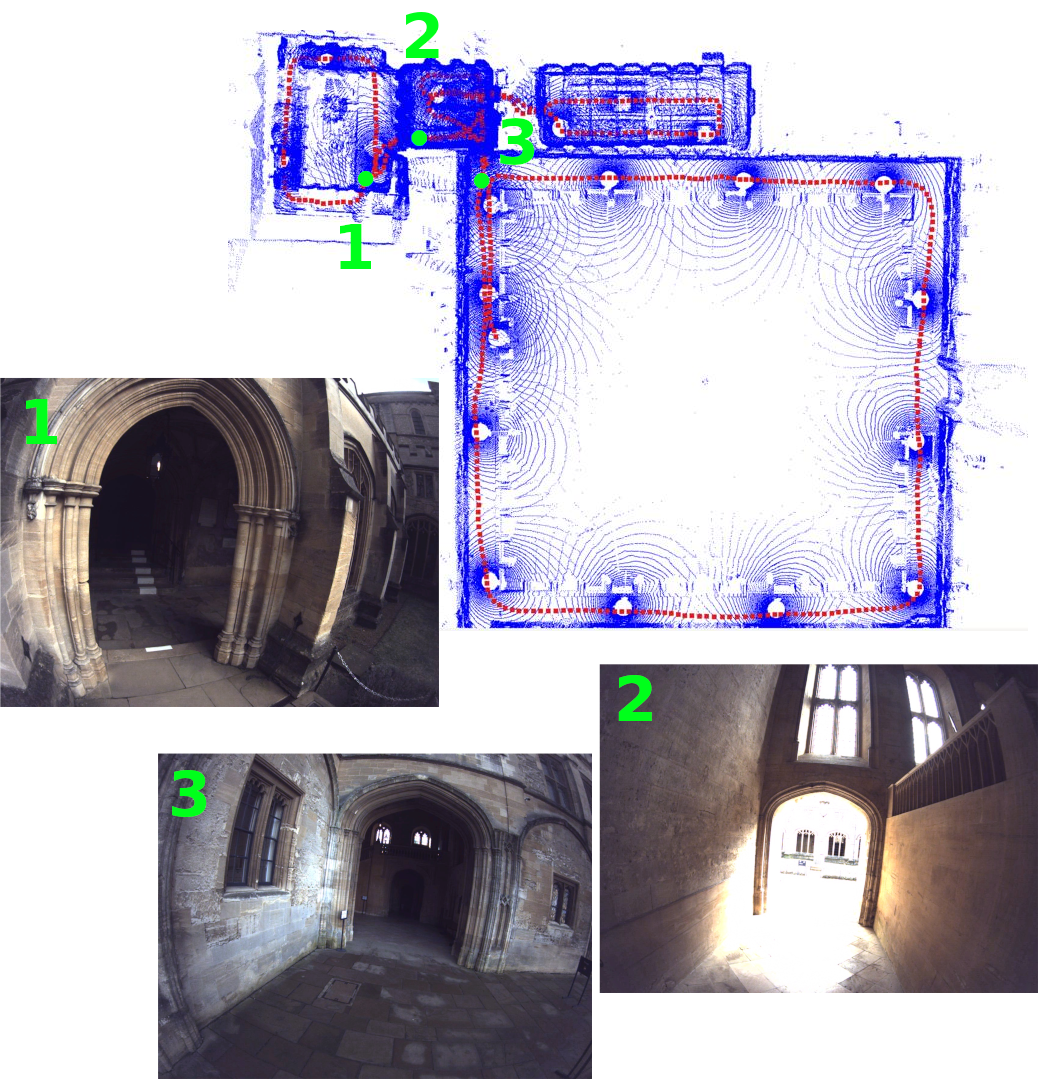
\includegraphics[width=0.8\linewidth]{fig/map_long_christ-church-02.png}
    \caption{Oxford Spires Dataset christ-church-02 sequences with a map visualizing example transition moments}
    \label{fig:map-christ-church-02}
\end{figure}

\begin{figure}[H]
    \centering
    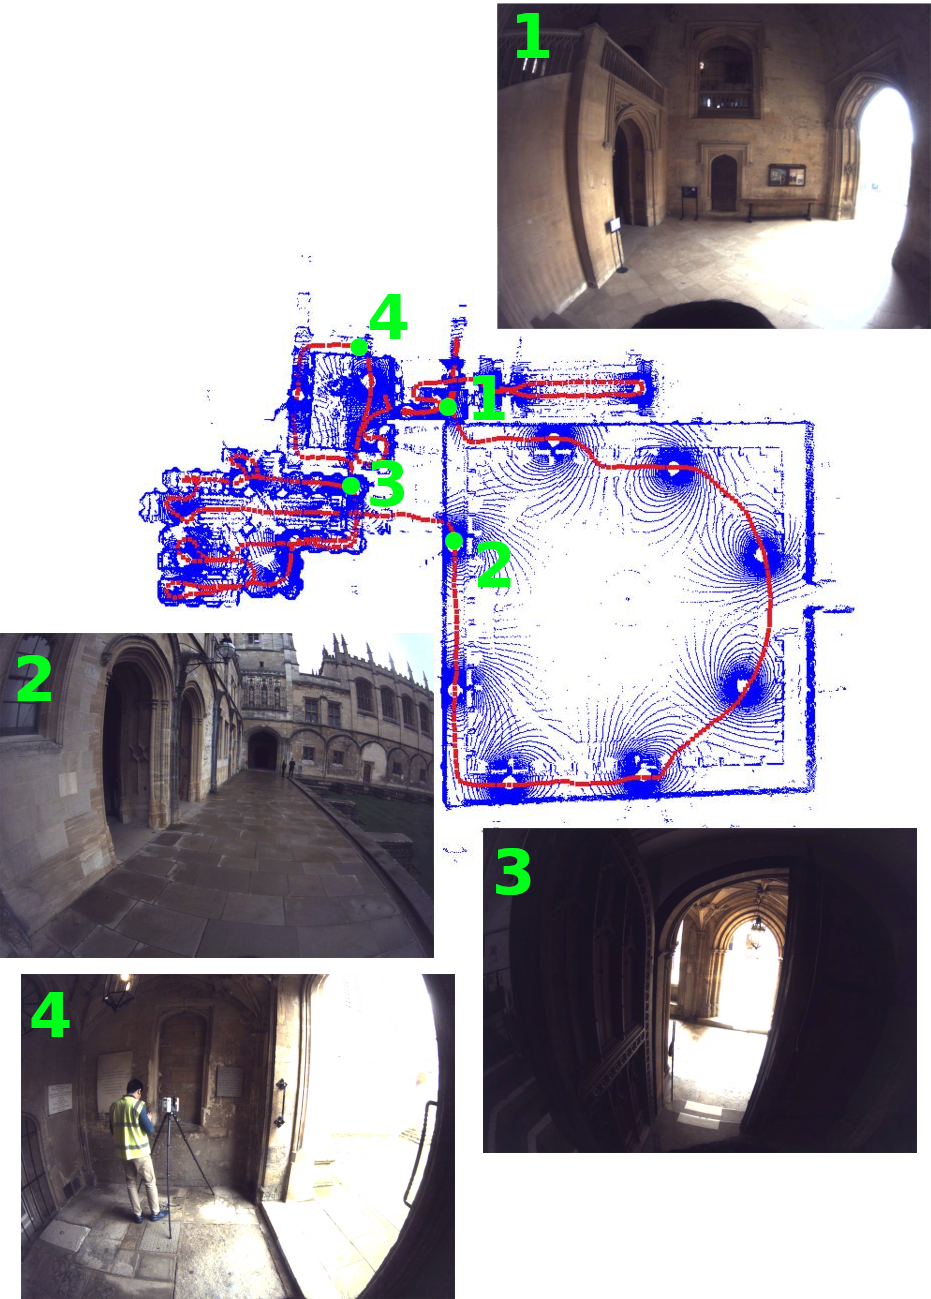
\includegraphics[width=0.8\linewidth]{fig/map_long_christ-church-05.png}
    \caption{Oxford Spires Dataset christ-church-05 sequences with a map visualizing example transition moments}
    \label{fig:map-christ-church-05}
\end{figure}




\subsection{Problem Statement}

Accurate and robust localization for mobile robots operating across mixed indoor–outdoor environments remains a significant challenge. This difficulty arises from rapid changes in visual appearance and geometry, coupled with intermittent or completely absent global positioning signals. Because individual sensors suffer from specific physical and environmental limitations—such as camera exposure saturation from outdoor glare or LiDAR geometric degeneracy in featureless corridors—relying on a single modality is insufficient for reliable autonomy. 

To overcome these vulnerabilities, autonomous systems must utilize sensor fusion to combine data from various sources, compensating for the limitations of each individual sensor and ensuring more accurate environmental perception. While contemporary computer vision and state estimation methods predominantly rely on datasets generated from cameras and LiDARs, this data is often augmented with GPS, IMU, Ultra-Wideband (UWB) ranging \cite{UWB-OptiTrack}, sonar, or magnetic field measurements \cite{magnetic_localzation} to allow for deeper condition interpretations and missing data recovery. 

Implementing this fusion, however, introduces distinct technical challenges. One prominent approach involves merging LiDAR and camera data to extract precise distance information for specific image pixels. To successfully combine this information, precise sensor extrinsic calibration between the camera and LiDAR is required to determine and maintain a common coordinate system. Furthermore, modern SLAM algorithms must fuse this multi-modal data to compute a highly accurate, continuous, and kinematically consistent transform chain ($map \rightarrow odom \rightarrow base\_link$) that does not rely on just one sensor.

The core problem addressed in this study is that while state-of-the-art sensor fusion and SLAM systems achieve sub-centimeter drift under strictly controlled, single-regime conditions, their performance during abrupt indoor–outdoor transitions remains underreported. From a probabilistic standpoint, these transitions—where fused modalities like GPS or stable visual features are suddenly lost or regained—cause a sudden inflation in the state covariance matrix, threatening the stability of the estimator. While recent comprehensive benchmark suites, such as MapsHD \cite{bedkowski2026mapshd}, have significantly advanced the automated qualitative and quantitative evaluation of LiDAR and LiDAR-inertial odometry frameworks, existing evaluations predominantly focus on long-term drift in static environments. They often fail to mathematically isolate and evaluate the transient ``stability shocks" caused by crossing these aggressive environmental thresholds.

\subsection{Contributions}
To address the challenges of seamless navigation in transitioning environments, this paper makes the following contributions:
\begin{itemize}
    \item \textbf{A Concise Review of State-of-the-Art (SOTA) Methods:} We provide a practitioner-oriented overview of localization approaches for mixed indoor–outdoor environments, categorizing filtering, optimization, and learning-based paradigms.
    \item \textbf{Empirical Evaluation and Benchmarking:} We present a comprehensive comparative analysis of six leading algorithms: FAST-LIO2 \cite{FAST-LIO2}, GLIM \cite{Koide_2024}, KISS-ICP \cite{KISS-ICP}, ORB-SLAM3 \cite{ORB-SLAM3}, RKO-LIO \cite{RKO-LIO}, and TSformer-VO \cite{franccani2025transformer}.
    \item \textbf{Granular Transition Analysis:} By leveraging the rich metadata of the Oxford Spires Dataset \cite{tao2025spires}, we \hl{apply a reproducible} temporal segmentation methodology \hl{with explicitly defined guard bands and transition windows} that isolates trajectory errors into strict indoor, strict outdoor, and transition-specific phases, revealing the exact vulnerabilities of each algorithm.
    \item \textbf{Reproducible Research Artifacts:} To support the robotics community and ensure reproducibility, we provide our optimized configuration files, sequence segmentation scripts, and parameter tunings used for the benchmarked algorithms\footnote{ \url{https://github.com/Cassie051/localization-benchamark}}.
\end{itemize}

%%%%%%%%%%%%%%%%%%%%%%%%%%%%%%%%%%%%%%%%%%
\section{Related Works and Background}
\label{sec:related}

State-of-the-art (SOTA) localization architectures leverage a diverse array of sensing modalities to perceive the environment and estimate the robot's state. Core modalities include Light Detection and Ranging (LiDAR) for precise geometric mapping, RGB and depth cameras for rich textural and structural information \cite{Visual-lidar}, Inertial Measurement Units (IMUs) for high-frequency kinematic measurements, and Global Navigation Satellite Systems (GNSS) for absolute positioning \cite{Robot-Localization-GNNS}. Major localization approaches have evolved to address the fusion of these modalities. Filter-based LiDAR-Inertial Odometry (LIO) systems, utilizing Extended Kalman Filters (EKF) and their iterative variants (ESIKF, IESKF), have become prominent for their computational efficiency and real-time performance \cite{FAST-LIO2}. In LIO, these can be further distinguished into loosely-coupled frameworks, which fuse subsystem outputs \cite{zhang2021coarse}, and tightly-coupled architectures that jointly estimate the state using LiDAR and IMU residuals \cite{bedkowski2026mapshd}.

In contrast, optimization-based SLAM frameworks employ factor graphs and scan-matching pipelines to jointly optimize poses, prioritizing accuracy and global consistency \cite{Koide_2024}. To bridge the gap between structure-less and feature-poor environments, Visual-LiDAR and multi-sensor fusion systems have emerged \cite{3d-2dlidar}, exploiting the complementary nature of optical and range data. In parallel, learning-based visual odometry has increasingly adopted transformer backbones inspired by video understanding architectures, enabling sequence-level motion modeling from monocular image streams \cite{franccani2025transformer,bertasius2021space,arnab2021vivit}. Synthesizing a unified approach that maintains robust performance during indoor-outdoor transitions, and validating it through rigorous open-source benchmarking tools \cite{BEDKOWSKI2024101618, bedkowski2026mapshd}, remains a critical challenge.

Robot localization relies on sensor perception and algorithms that determine how a pose is calculated \cite{Borenstein1996WhereAI}. Integrating a higher number of sensors provides data redundancy, which significantly increases the robustness of the positioning system. In mixed indoor–outdoor environments, selecting the appropriate sensor suite is critical for maintaining reliability across differing conditions. Indoor areas consist of corridors, walls, ceilings, structured rooms, and stable lighting. Conversely, outdoor areas often feature vast distances, changing weather and lighting conditions, buildings, and vegetation. These varied and challenging conditions significantly impact algorithmic performance. A sudden lack of high-frequency geometric constraints negatively affects the covariance matrix of the state estimate for the predicted pose.

To systematically categorize these diverse architectures, Table~\ref{classification-localization-methods} presents a comprehensive taxonomy of mobile robot localization methods. It classifies current methodologies across three primary dimensions: the underlying sensor modalities (proprioceptive, exteroceptive, or absolute), the spatial scope of the localization (ranging from local odometry to global positioning), and the core mathematical estimation paradigms utilized to compute the state.

\begin{table}[h]   
    \centering
    \caption{Taxonomy of Mobile Robot Localization Methods}
    \label{classification-localization-methods}
    \begin{tabular}{p{4cm} p{4cm} p{4cm}}
        \toprule
        \toprule
        \textbf{Sensor Modality} & 
        \textbf{Localization Scope} & 
        \textbf{Estimation Paradigm} \\ 
        \midrule
        \midrule
        
        \textbf{Proprioceptive} \newline \newline \footnotesize{IMU, \newline Wheel Encoders} 
        & 
        \textbf{Local} \newline \newline \footnotesize{Odometry, \newline Dead Reckoning}
        & 
        \textbf{Filter-Based} \newline \newline \footnotesize{EKF, ESIKF, \newline Particle Filters (MCL)} \\
        \midrule
        
        \textbf{Exteroceptive} \newline \newline \footnotesize{LiDAR (2D/3D), Cameras (RGB/D, Thermal), Radar}
        & 
        \textbf{Simultaneous (SLAM)} \newline \newline \footnotesize{Joint trajectory \& map estimation}
        & 
        \textbf{Optimization-Based} \newline \newline \footnotesize{Factor Graphs, Sliding Window, Bundle Adjustment} \\
        \midrule
        
        \textbf{Absolute} \newline \newline \footnotesize{GNSS, UWB~\cite{UWB-OptiTrack}, \newline IR Beacons, \newline Magnetic \cite{magnetic_localzation}}
        & 
        \textbf{Global} \newline \newline \footnotesize{Prior map matching, \newline Satellite positioning}
        & 
        \textbf{Learning-Based} \newline \newline \footnotesize{CNNs,\newline Transformer-based odometry} \\
        
        \bottomrule
        \bottomrule
    \end{tabular}
\end{table}

When a specific sensor becomes unreliable, the system must compensate for corrupted or missing data through robust fusion algorithms. While vision-based systems are popular, they often struggle in outdoor environments where a lack of distinct features or lighting changes can degrade positioning accuracy. Consequently, the fusion of LiDAR and IMU data has emerged as a state-of-the-art solution for providing accurate and robust positioning during the complex transitions between indoor and outdoor spaces \cite{FAST-LIO2, shan2020liosam, nubert2021self}.

\hl{A complementary line of research, developed mainly in the context of seamless pedestrian and smartphone navigation, addresses the automatic recognition of the operating environment itself}~\cite{feriol2020review} \hl{. IODetector}~\cite{zhou2012iodetector} \hl{infers whether a~device is indoors or outdoors from light intensity, magnetic field variance, and cellular signal strength, without any prior fingerprinting of the environment. Zhu et al.}~\cite{zhu2019fastio} \hl{apply machine-learning classifiers to detect indoor/outdoor transitions quickly, reducing the switching delay in transition regions. SUNS}~\cite{mansour2022suns} \hl{extends this concept to an enhanced indoor--outdoor environmental awareness service that acts as an automatic handover mechanism between positioning sources (GNSS, Wi-Fi, and inertial sensors) within an extended Kalman filter. These approaches recognize the environment online in order to select or re-weight positioning sources. In contrast, the segmentation used in this study is an offline evaluation tool: indoor, outdoor, and transition labels are assigned to dataset timestamps in order to measure how unmodified localization algorithms behave in each regime. The two lines of work are complementary: the transition-specific failure modes identified here indicate where an environment-aware handover or re-weighting mechanism would be most beneficial for LiDAR- and camera-based robot localization, and they motivate the adaptive multimodal fusion discussed in Section}~\ref{sec:conclusions}.

%%%%%%%%%%%%%%%%%%%%%%%%%%%%%%%%%%%%%%%%%%
\section{Methodology}

The methodology of this study follows a systematic pipeline designed to evaluate the operational limits of multi-sensor fusion in transitioning environments. The research logic is divided into three primary phases: algorithmic selection, trajectory segmentation, and targeted benchmarking. 

Initially, the selection of the algorithms was determined by the sensor modalities—specifically the availability of high-frequency Inertial Measurement Units (IMU), multi-beam LiDAR, and visual cameras. By choosing frameworks that represent distinct mathematical paradigms (recursive filtering, factor graph optimization, \hl{monocular visual-inertial optimization}, and direct scan-to-map registration), we aim to identify which architecture maintains the highest stability during the geometric and lighting shocks of indoor–outdoor transitions. 

The selected algorithms were open-source, demonstrated high accuracy as declared by their authors, and served as state-of-the-art deterministic baselines (in the case of ORB-SLAM3 and KISS-ICP). However, due to various algorithmic limitations—such as an inability to run in real-time, sensor applicability mismatches, or hardware and software compatibility issues—several frameworks, such as those proposed in \cite{BEDKOWSKI2024101618} and \cite{nubert2021self}, could not be successfully applied and compared in this study.

\subsection{Dataset and Environmental Segmentation}
The empirical evaluation was conducted using the Oxford Spires Dataset \cite{tao2025spires}, which provides continuous recordings of a sensor rig traversing highly complex historical university environments. This dataset was selected due to its high-precision terrestrial laser-scanning ground-truth and its inclusion of indoor-outdoor transition data. 

To isolate the impact of environmental changes on localization stability, the continuous sequences—specifically \texttt{2024-03-20-christ-church-05} (Seq 05) and \hl{\texttt{2024-03-18-christ-church-02}} (Seq 02) were temporally segmented into three distinct categories: \textit{Indoor}, \textit{Outdoor}, and \textit{Transition} (Indoor-Outdoor). The visualization of divided trajectories for categories in each sequences are presented in Fig. \ref{fig:trajectory_splits}.

This segmentation was achieved by analyzing the dataset's metadata, LiDAR measurements, and camera images. Based on the data records, exact timestamps when the sensor rig crossed structural boundaries were defined. Specifically, timestamps corresponding to narrow doorways allowed us to determine:
\begin{itemize}
    \item \textbf{Indoor/Outdoor Phases:} Computed as the periods strictly occurring between boundary crossings, ensuring the algorithms were exposed to fully enclosed structures or fully open areas.
    \item \textbf{Transition Phases:} To capture the ``stability shock", the transitional segments were defined as the immediate temporal windows surrounding the threshold crossings (e.g. exiting a doorway). This isolates the exact moments where algorithms must renegotiate sensor confidence, handle sudden feature loss, or recover from intense illumination changes.
\end{itemize}

\begin{figure*}
\begin{subfigure}{\textwidth}
  \centering
  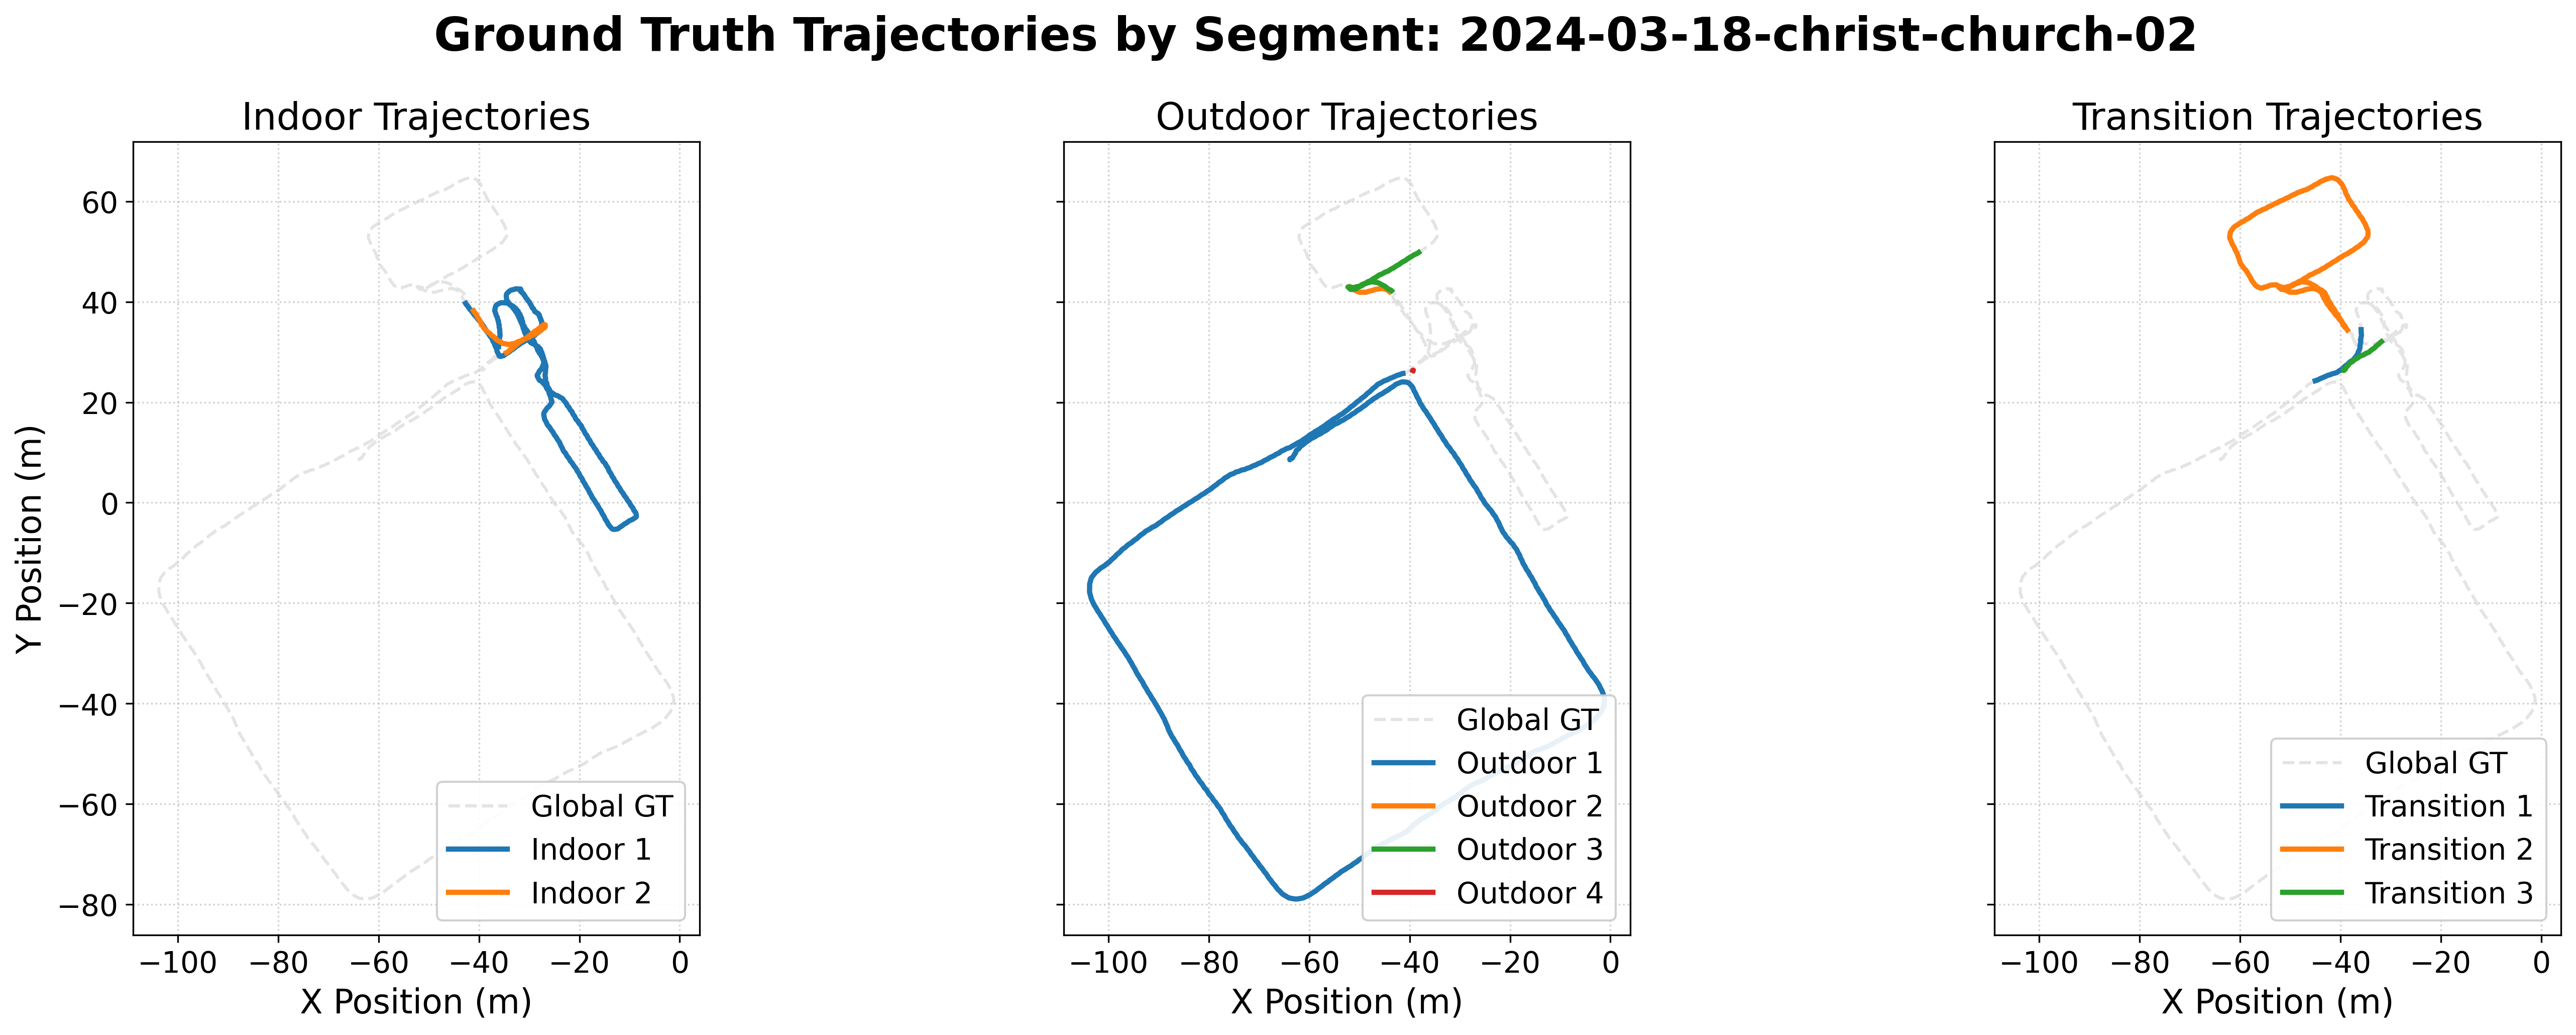
\includegraphics[width=\linewidth]{fig/trajectory_splits_christ-church-02.png}
  \label{fig:trajectory_splits_christ-church-02}
\end{subfigure}
    \hfill%
\begin{subfigure}{\textwidth}
  \centering
  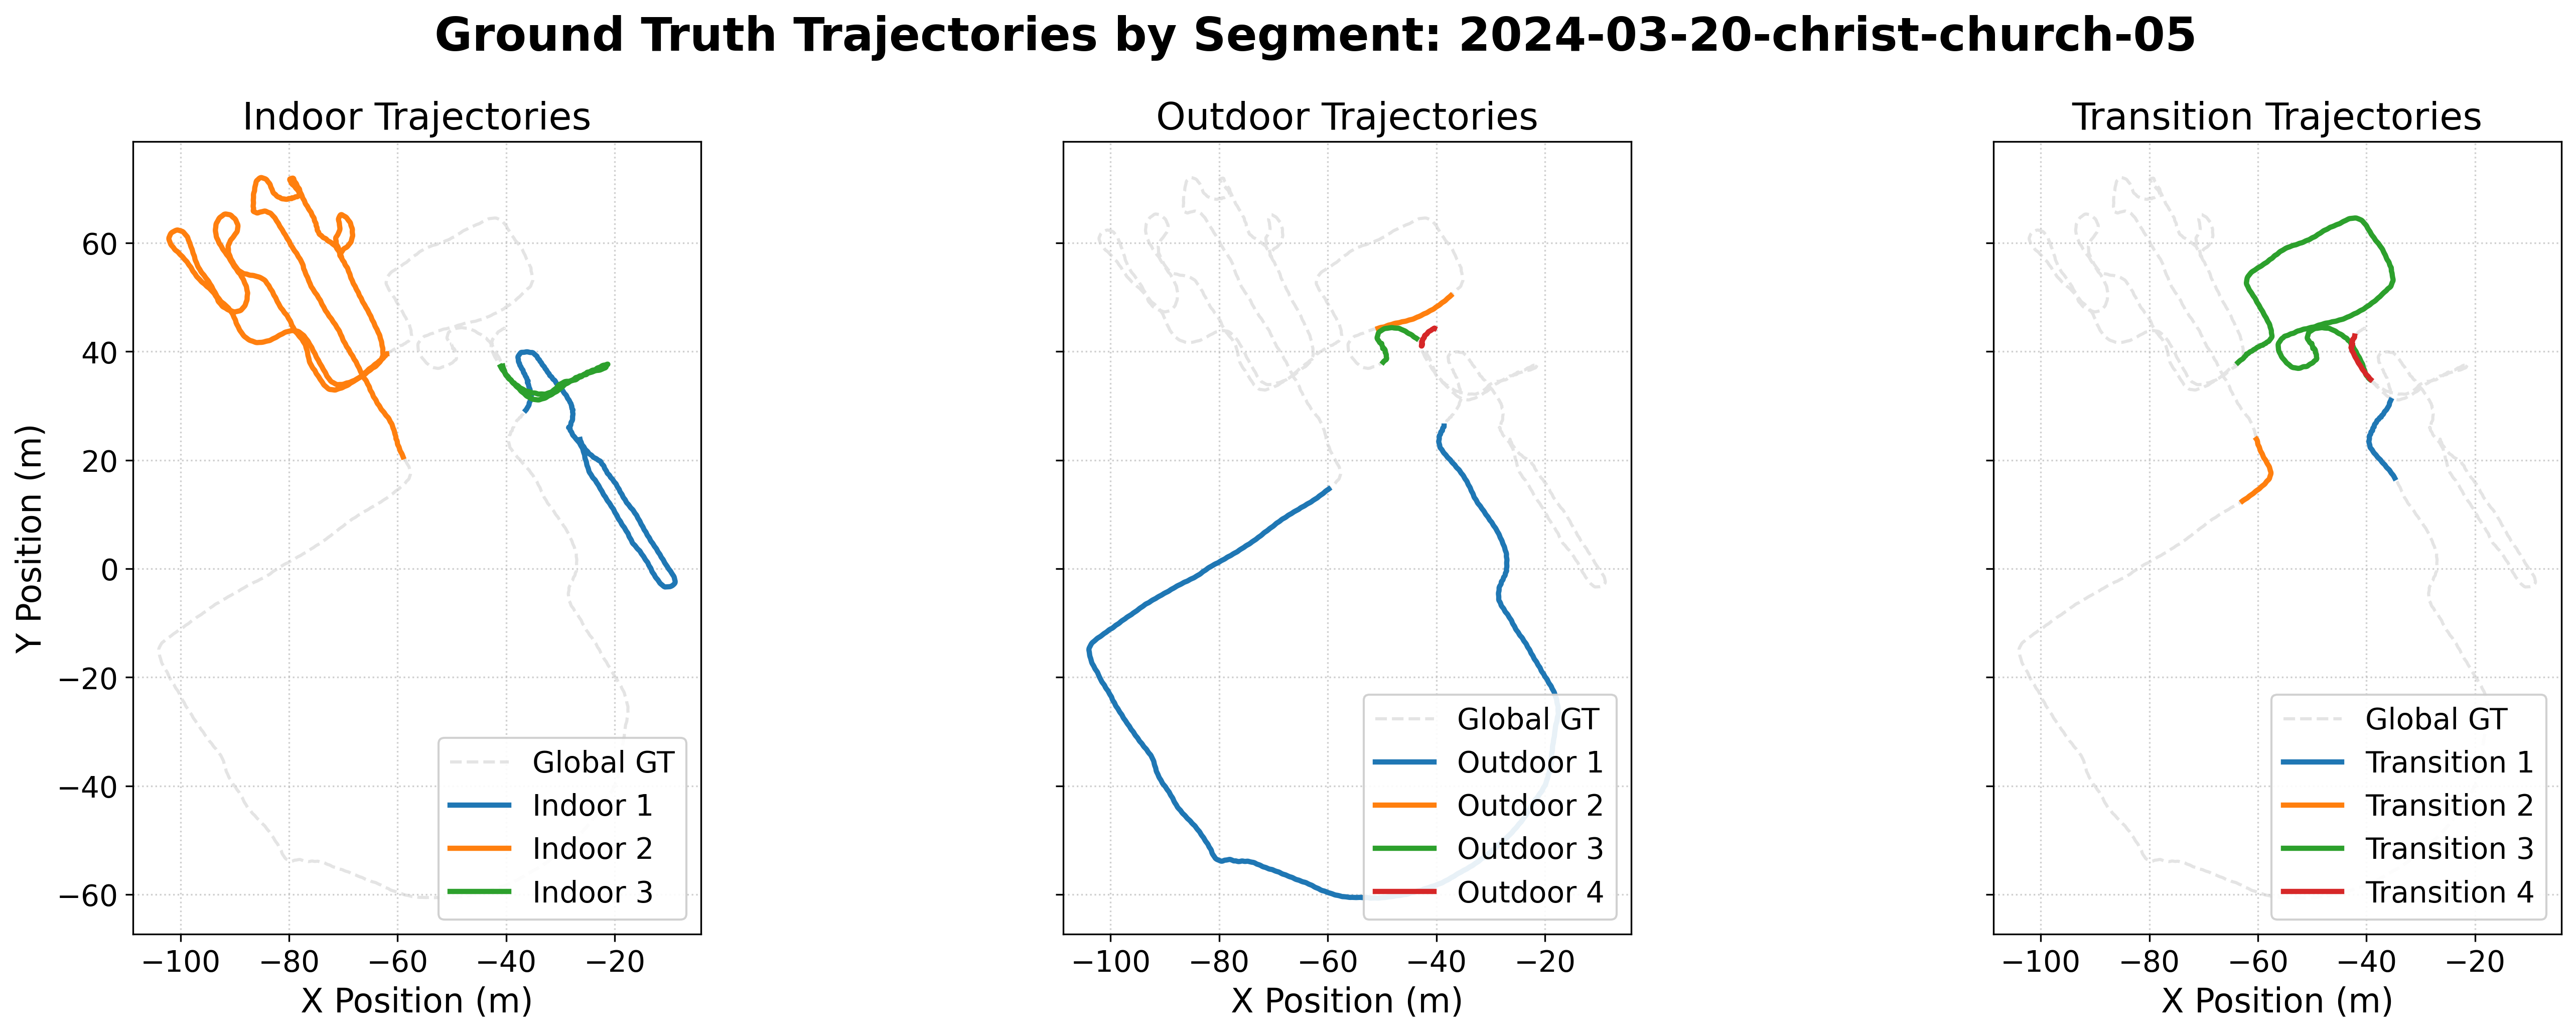
\includegraphics[width=\linewidth]{fig/trajectory_splits_christ-church-05.png}
  \label{fig:trajectory_splits_christ-church-05}
\end{subfigure}
\caption{Trajectory splits for Indoor, Outdoor, and Transition (Indoor-Outdoor) regimes for the tested sequences.}
\label{fig:trajectory_splits}
\end{figure*}

\subsection{Algorithms Configuration}
To ensure a rigorous and fair empirical comparison, the configuration files of all evaluated algorithms were meticulously adapted to interface with the provided Oxford Spires Dataset ROS bag formats. A critical step in this preparation involved applying the dataset's native extrinsic calibrations---specifically the structural translations and rotations between the LiDAR and the IMU. This guaranteed that all physical sensor measurements were accurately projected into a unified coordinate frame across all tested frameworks. Furthermore, the purely visual-inertial baseline, ORB-SLAM3, required specific dataset-tailored adaptations. Its configuration was explicitly modified to correctly ingest the Oxford Spires camera models, image streams, and synchronization data, allowing it to be seamlessly executed and evaluated alongside the predominantly LiDAR-based odometry systems.

\subsection{Learning-Based Baseline Model (TSformer-VO)}

TSformer-VO is an end-to-end artificial intelligence-based model designed for monocular visual odometry. It represents a modern research direction that leverages deep learning models to estimate camera motion from image sequences, providing an alternative to the classical geometry-based methods commonly employed in robot navigation. The model estimates the camera's position and orientation in three-dimensional space by analyzing consecutive image frames captured by a monocular camera. Unlike conventional visual odometry methods and SLAM systems, TSformer-VO formulates motion estimation not as a purely geometric problem but as a video understanding task. The model processes consecutive image frames and directly estimates the relative camera motion between them without explicitly detecting and matching visual features \cite{franccani2025transformer}.

Before deployment, the model must undergo a supervised learning process. During training, the network parameters are optimized by minimizing a loss function that quantifies the discrepancy between the estimated and the ground-truth trajectories. Once trained, the model can be used to estimate camera motion in previously unseen environments.

To avoid data leakage while still enabling evaluation on both target routes, two separate TSformer-VO models were trained. One model was trained on all selected Oxford Spires sequences with available ground-truth poses except \texttt{christ\_church\_02}, and the second model used the same training pool except \texttt{christ\_church\_05}. In each case, the excluded route was used only for final testing.

For validation, we used cyclic sequence-level cross-validation during training: at each epoch, one full training sequence was selected as validation and the remaining sequences were used for optimization. This protocol preserves temporal coherence within each route and avoids mixing samples from the same route between train and validation within an epoch.

Input images were generated from Oxford Spires trajectories downsampled from 20 Hz to 5 Hz to match the \texttt{christ\_church\_05} acquisition rate. Ground-truth poses were matched to image timestamps using nearest-neighbor timestamp association. All frames were resized to $192\times640$ and normalized with fixed RGB mean/std values. No data augmentation was applied.

Model initialization used the authors' pretrained TSformer checkpoint \texttt{checkpoint\_model1\_exp12}. The predicted output is a flattened vector of relative poses for each temporal window ($6\times(\texttt{window\_size}-1)$), with supervision built from relative SE(3) motion between consecutive matched frames, represented as Euler angles plus translation and normalized using fixed statistics.

Optimization used Adam with batch size $8$, learning rate $10^{-5}$, momentum $0.9$, weight decay $10^{-4}$, and up to $100$ epochs. The loss was MSE on the pose vector, with model selection based on best validation loss. Training was performed on one NVIDIA A100 40 GiB GPU with 64 GB RAM allocation; the approximate training time was 44 hours.

\subsection{Metrics}
To quantify localization accuracy across the segmented phases, our evaluation employs two complementary metrics: Relative Pose Error (RPE) and Absolute Pose Error (APE). While RPE is specifically designed to capture local trajectory consistency and frame-to-frame tracking accuracy over fixed intervals, APE measures the global drift and absolute trajectory deviation from the ground truth within that segment \cite{grupp2017evo}. 

The relative pose error matrix for a time step $i$ over a fixed spatial or temporal interval $\Delta t$ is defined mathematically by aligning the estimated and reference relative transformations:
\begin{equation}
  \begin{gathered}
    \mathbf{E}_{RPE,i} = \left( \mathbf{T}_{ref,i}^{-1} \mathbf{T}_{ref,i+\Delta t} \right)^{-1} 
    \left( \mathbf{T}_{est,i}^{-1} \mathbf{T}_{est,i+\Delta t} \right) \in SE(3)
\end{gathered}
\end{equation}
Conversely, the absolute pose error evaluates the global consistency of the estimated pose:
\begin{equation}
    \mathbf{E}_{APE,i} = \mathbf{T}_{ref,i}^{-1} \mathbf{T}_{est,i} \in SE(3)
\end{equation}

To determine the exact positional error for each discrete state, we extract the $L_2$ norm of the translation component from the error matrices. This yields the point-wise Euclidean distance error for that specific local frame:
\begin{equation}
    e_i = \left\| \text{trans}(\mathbf{E}_i) \right\|_2
\end{equation}

Finally, to aggregate these exact point-wise errors over a specific segmented patch (e.g., an indoor corridor or an outdoor courtyard) containing $N$ poses, we extract two summary statistics. The Root Mean Square Error (RMSE) is computed to evaluate the overall expected accuracy:
\begin{equation}
    RMSE = \sqrt{\frac{1}{N} \sum_{i=1}^{N} e_i^2}
\end{equation}
Additionally, we record the Maximum Error ($Max = \max_{i=1}^{N} e_i$) to capture instantaneous, severe tracking divergences or ``stability shocks." By calculating both RMSE and Max statistics across isolated Indoor, Outdoor, and Transition segments, we can objectively identify algorithmic vulnerabilities that are typically obscured when looking only at full-trajectory averages.

%%%%%%%%%%%%%%%%%%%%%%%%%%%%%%%%%%%%%%%%%%
\section{Results}
The empirical results are divided into three distinct operational phases: strictly indoor, strictly outdoor, and the transition threshold. To highlight the most robust frameworks, the best-performing (lowest error) algorithm for each specific segment and the overall average are marked in \textbf{bold}.

\subsection{Indoor Environments}

% ==================================================
% CATEGORY GROUP: INDOOR
% ==================================================
% --- Indoor Combined Table (RPE) ---
\begin{table*}[!ht]
\caption{Detailed RPE Metrics (RMSE and Max in m) for Indoor Environments (Combined Seq 02 \& 05)}
\label{tab:results-indoor-rpe}
\resizebox{\textwidth}{!}{
\begin{tabular}{llccccccc}
\toprule
\toprule
\multirow{2}{*}{Algorithm} & \multirow{2}{*}{Metric} & \multicolumn{2}{c}{Seq 02} & \multirow{2}{*}{Average} & \multicolumn{3}{c}{Seq 05} & \multirow{2}{*}{Average} \\
\cmidrule(lr){3-4} \cmidrule(lr){6-8}
 & & Indoor 1 & Indoor 2 & & Indoor 1 & Indoor 2 & Indoor 3 & \\
\midrule
\midrule
\multirow{2}{*}{FASTLIO} 
 & RMSE & 9.792 & 0.036 & 4.914 & 0.055 & 0.183 & 0.061 & 0.099 \\
 & Max  & 82.401 & 0.097  & - & 0.563 & 2.137 & 0.191 & - \\
\cmidrule(lr){1-9}

\multirow{2}{*}{GLIM} 
 & RMSE & \textbf{0.023} & \textbf{0.022} & \textbf{0.022} & \textbf{0.033} & \textbf{0.020} & \textbf{0.042} & \textbf{0.032} \\
 & Max  & \textbf{0.139} & \textbf{0.060}  & - & \textbf{0.102} & 0.163 & \textbf{0.113} & - \\
\cmidrule(lr){1-9}

\multirow{2}{*}{KISS\_ICP} 
 & RMSE & 0.169 & 0.138  & 0.153 & 0.145 & 0.139 & 0.167 & 0.150 \\
 & Max  & 0.730 & 0.412 & - & 0.591 & 0.652 & 0.622 & - \\
\cmidrule(lr){1-9}

\multirow{2}{*}{ORB-SLAM3} 
 & RMSE & 0.102 & 0.158  & 0.130 & 0.263 & 0.333 & 0.445 & 0.347 \\
 & Max  & 4.421 & 3.176 & - & 1.824 & 5.253 & 4.376 & - \\
\cmidrule(lr){1-9}

\multirow{2}{*}{RKO\_LIO} 
 & RMSE & 0.040 & 0.043  & 0.042 & 0.044 & 0.033 & 0.053 & 0.043 \\
 & Max  & 0.140 & 0.115  & - & 0.115 & \textbf{0.131} & 0.271 & - \\
\cmidrule(lr){1-9}

\multirow{2}{*}{TSformer-VO} 
 & RMSE & 0.069 & 0.073 & 0.071 & 0.067 & 0.069 & 0.088 & 0.075 \\
 & Max  & 0.235 & 0.189 & - & 0.237 & 0.455 & 0.526 & - \\
\bottomrule
\bottomrule
\end{tabular}
}
\end{table*}

% --- Indoor Combined Table (APE) ---
\begin{table*}[!ht]
\caption{Detailed APE Metrics (RMSE and Max in m) for Indoor Environments (Combined Seq 02 \& 05)}
\label{tab:results-indoor-ape}
\resizebox{\textwidth}{!}{
\begin{tabular}{llccccccc}
\toprule
\toprule
\multirow{2}{*}{Algorithm} & \multirow{2}{*}{Metric} & \multicolumn{2}{c}{Seq 02} & \multirow{2}{*}{Average} & \multicolumn{3}{c}{Seq 05} & \multirow{2}{*}{Average} \\
\cmidrule(lr){3-4} \cmidrule(lr){6-8}
 & & Indoor 1 & Indoor 2  & & Indoor 1 & Indoor 2 & Indoor 3 & \\
\midrule
\midrule
\multirow{2}{*}{FASTLIO} 
 & RMSE & 1885.176 & 0.225  & 942.701 & 1.496 & 17.560 & 0.559 & 6.538 \\
 & Max  & 5914.812 & 0.482  & - & 3.488 & 28.949 & 1.586 & - \\
\cmidrule(lr){1-9}

\multirow{2}{*}{GLIM} 
 & RMSE & 0.126 & \textbf{0.038} & 0.082 & \textbf{0.040} & 0.085 & \textbf{0.060} & 0.062 \\
 & Max  & 0.374 & \textbf{0.085} & - & \textbf{0.099} & \textbf{0.240} & \textbf{0.159} & - \\
\cmidrule(lr){1-9}

\multirow{2}{*}{KISS\_ICP} 
 & RMSE & 0.211 & 0.176 & 0.193 & 0.173 & 0.197 & 0.228 & 0.199 \\
 & Max  & 0.792 & 0.343 & - & 0.702 & 0.744 & 0.672 & - \\
\cmidrule(lr){1-9}

\multirow{2}{*}{ORB-SLAM3} 
 & RMSE & 0.514 & 0.616 & 0.565 & 0.482 & 0.593 & 2.130 & 1.068 \\
 & Max  & 3.669 & 2.973 & - & 2.928 & 5.789 & 8.057 & - \\
\cmidrule(lr){1-9}

\multirow{2}{*}{RKO\_LIO} 
 & RMSE & \textbf{0.110} & 0.052  & \textbf{0.081} & 0.046 & \textbf{0.058} & 0.071 & \textbf{0.058} \\
 & Max  & \textbf{0.283} & 0.127  & - & 0.155 & 0.279 & 0.204 & - \\
\cmidrule(lr){1-9}

\multirow{2}{*}{TSformer-VO} 
 & RMSE & 7.264 & 1.918 & 4.591 & 8.329 & 13.699 & 5.054 & 9.027 \\
 & Max  & 20.492 & 4.315 &  - & 22.650 & 31.691 & 9.369 & - \\
\bottomrule
\bottomrule
\end{tabular}
}
\end{table*}
In strictly indoor environments (Tables~\ref{tab:results-indoor-rpe},\ref{tab:results-indoor-ape}), the optimization-based \textbf{GLIM} framework demonstrates the most consistent performance, achieving the best overall average RPE RMSE ($0.022$ m in Seq 02 and $0.032$ m in Seq 05). This superior local consistency translates to exceptional global stability, as GLIM also records the lowest APE Max values (averaging just $0.166$ m in Seq 05). This stability can be attributed to its GPU-accelerated factor graph, which excels at registering point clouds against structured geometric constraints such as walls and corridors. 

\textbf{RKO-LIO} closely follows as the second-best, maintaining a highly stable average RPE RMSE of $0.042$ m and $0.043$ m across both sequences. Notably, FAST-LIO2 experienced a catastrophic tracking failure in the first indoor segment of Sequence 02; while its local RPE spiked to a maximum of $82.401$ m, its global APE Max diverged completely, exceeding $5900$ m. Meanwhile, the purely visual ORB-SLAM3 saw its performance severely degrade, particularly in Sequence 05 (averaging $0.347$ m in RPE RMSE and reaching up to $8.057$ m in APE Max), highlighting the vulnerability of cameras to featureless walls and motion blur. TSformer-VO maintained competitive local indoor tracking (RPE RMSE averages of $0.071$ m in Seq 02 and $0.075$ m in Seq 05), but exhibited substantially larger global drift, with APE RMSE averages of $4.591$ m and $9.027$ m and APE Max peaks up to $31.691$ m.



\subsection{Outdoor Environments}


When navigating wide-baseline outdoor environments (Tables~\ref{tab:results-outdoor-rpe}, \ref{tab:results-outdoor-ape}), \textbf{GLIM} again secures the best overall stability with an average RPE RMSE of $0.024$ m (Seq 02) and $0.039$ m (Seq 05), dominating almost all individual patches. FAST-LIO2 also demonstrated excellent frame-to-frame performance, particularly in Sequence 02 ($0.033$ m average RPE RMSE). However, it experienced a massive tracking deviation in the third segment of Sequence 05; while the RPE RMSE showed an anomaly ($1.114$ m), the APE Max reveals the true scale of the failure, registering a $44.846$ m global drift. 

% ==================================================
% CATEGORY GROUP: OUTDOOR
% ==================================================

% --- Outdoor Combined Table (RPE) ---
\begin{table*}[h]
\caption{Detailed RPE Metrics (RMSE and Max in m) for Outdoor Environments (Combined Seq 02 \& 05)}
\label{tab:results-outdoor-rpe}
\resizebox{\textwidth}{!}{
\begin{tabular}{llcccccccccc}
\toprule
\toprule
\multirow{2}{*}{Algorithm} & \multirow{2}{*}{Metric} & \multicolumn{4}{c}{Seq 02} & \multirow{2}{*}{Average} & \multicolumn{4}{c}{Seq 05} & \multirow{2}{*}{Average} \\
\cmidrule(lr){3-6} \cmidrule(lr){8-11}
 & & Outdoor 1 & Outdoor 2 & Outdoor 3 & Outdoor 4 & & Outdoor 1 & Outdoor 2 & Outdoor 3 & Outdoor 4 & \\
\midrule
\midrule
\multirow{2}{*}{FASTLIO} 
 & RMSE & \textbf{0.037} & 0.048 & 0.038 & 0.009 & 0.033 & 0.037 & 0.090 & 1.114 & 0.028 & 0.317 \\
 & Max  & \textbf{0.196} & 0.208 & 0.225 & 0.029 & - & 0.162 & \textbf{0.141} & 3.382 & 0.133 & - \\
\cmidrule(lr){1-12}

\multirow{2}{*}{GLIM} 
 & RMSE & 0.042 & \textbf{0.026} & \textbf{0.019} & \textbf{0.008} & \textbf{0.024} & \textbf{0.028} & \textbf{0.088} & \textbf{0.027} & \textbf{0.014} & \textbf{0.039} \\
 & Max  & 0.393 & \textbf{0.083} & \textbf{0.062} & \textbf{0.019} & - & 0.191 & 0.147 & \textbf{0.069} & \textbf{0.073} & - \\
\cmidrule(lr){1-12}

\multirow{2}{*}{KISS\_ICP} 
 & RMSE & 0.262 & 0.142 & 0.165 & 0.044 & 0.153 & 0.303 & 0.150 & 0.180 & 0.125 & 0.190 \\
 & Max  & 1.037 & 0.268 & 0.415 & 0.115 & - & 1.438 & 0.269 & 0.425 & 0.376 & - \\
\cmidrule(lr){1-12}

\multirow{2}{*}{ORB-SLAM3} 
 & RMSE & 0.111 & 0.190 & 0.179 & - & 0.160 & 0.356 & 0.695 & 0.744 & 0.213 & 0.502 \\
 & Max  & 3.385 & 2.012 & 3.196 & - & - & 4.326 & 4.375 & 3.573 & 0.613 & - \\
\cmidrule(lr){1-12}

\multirow{2}{*}{RKO\_LIO} 
 & RMSE & 0.058 & 0.046 & 0.049 & 0.027 & 0.045 & 0.043 & 0.096 & 0.037 & 0.040 & 0.054 \\
 & Max  & 0.278 & 0.101 & 0.193 & 0.092 & - & \textbf{0.144} & 0.164 & 0.087 & 0.110 & - \\
\cmidrule(lr){1-12}

\multirow{2}{*}{TSformer-VO} 
 & RMSE & 0.064 & 0.066 & 0.066 & 0.193 & 0.097 & 0.058 & 0.050 & 0.105 & 0.135 & 0.087 \\
 & Max  & 0.267 & 0.174 & 0.201 & 0.247 & - & 0.226 & 0.079 & 0.288 & 0.231 & - \\
\bottomrule
\bottomrule
\end{tabular}
}
\end{table*}

% --- Outdoor Combined Table (APE) ---
\begin{table*}[h]
\caption{Detailed APE Metrics (RMSE and Max in m) for Outdoor Environments (Combined Seq 02 \& 05)}
\label{tab:results-outdoor-ape}
\resizebox{\textwidth}{!}{
\begin{tabular}{llcccccccccc}
\toprule
\toprule
\multirow{2}{*}{Algorithm} & \multirow{2}{*}{Metric} & \multicolumn{4}{c}{Seq 02} & \multirow{2}{*}{Average} & \multicolumn{4}{c}{Seq 05} & \multirow{2}{*}{Average} \\
\cmidrule(lr){3-6} \cmidrule(lr){8-11}
 & & Outdoor 1 & Outdoor 2 & Outdoor 3 & Outdoor 4 & & Outdoor 1 & Outdoor 2 & Outdoor 3 & Outdoor 4 & \\
\midrule
\midrule
\multirow{2}{*}{FASTLIO} 
 & RMSE & 1.046 & 0.145 & 0.209 & \textbf{0.010} & 0.353 & 0.625 & \textbf{0.055} & 15.623 & 0.144 & 4.112 \\
 & Max  & 1.948 & 0.340 & 0.474 & 0.029 & - & 1.761 & \textbf{0.114} & 44.846 & 0.232 & - \\
\cmidrule(lr){1-12}

\multirow{2}{*}{GLIM} 
 & RMSE & 1.710 & \textbf{0.029} & \textbf{0.036} & 0.012 & 0.447 & \textbf{0.059} & 0.055 & 0.046 & \textbf{0.026} & \textbf{0.046} \\
 & Max  & 4.290 & \textbf{0.069} & \textbf{0.102} & \textbf{0.024} & - & \textbf{0.156} & 0.129 & 0.135 & \textbf{0.068} & - \\
\cmidrule(lr){1-12}

\multirow{2}{*}{KISS\_ICP} 
 & RMSE & 0.313 & 0.133 & 0.198 & 0.056 & 0.175 & 0.317 & 0.131 & 0.185 & 0.156 & 0.198 \\
 & Max  & 1.035 & 0.238 & 0.529 & 0.108 & - & 1.597 & 0.253 & 0.412 & 0.372 & - \\
\cmidrule(lr){1-12}

\multirow{2}{*}{ORB-SLAM3} 
 & RMSE & 1.994 & 0.568 & 0.661 & - & 1.074 & 1.493 & 1.904 & 2.396 & 0.905 & 1.674 \\
 & Max  & 4.859 & 1.724 & 2.754 & - & - & 10.145 & 4.212 & 3.819 & 1.430 & - \\
\cmidrule(lr){1-12}

\multirow{2}{*}{RKO\_LIO} 
 & RMSE & \textbf{0.138} & 0.038 & 0.050 & 0.041 & \textbf{0.067} & 0.098 & 0.067 & \textbf{0.044} & 0.053 & 0.066 \\
 & Max  & \textbf{0.539} & 0.078 & 0.148 & 0.104 & - & 0.264 & 0.159 & \textbf{0.098} & 0.149 & - \\
\cmidrule(lr){1-12}

\multirow{2}{*}{TSformer-VO} 
 & RMSE & 8.860 & 0.302 & 2.307 & 3.822 & 3.823 & 19.464 & 0.242 & 0.964 & 2.457 & 5.782 \\
 & Max  & 19.424 & 0.536 & 5.709 & 6.570 & - & 52.145 & 0.521 & 2.030 & 4.975 & - \\
\bottomrule
\bottomrule
\end{tabular}
}
\end{table*}

In contrast to the LiDAR-inertial methods, the purely visual ORB-SLAM3 struggled significantly in unstructured terrain, dropping a segment in Sequence 02 and yielding the highest tracking errors in Sequence 05 (reaching an APE Max of $10.145$ m). The LiDAR-inertial methods (especially GLIM and RKO-LIO) maintained much tighter, predictable error bounds across both sequences, showcasing the reliability of fusing high-frequency IMU data with 3D structural geometry over wide areas. TSformer-VO achieved moderate local consistency outdoors (RPE RMSE averages of $0.097$ m for Seq 02 and $0.087$ m for Seq 05), yet its global drift remained elevated, with APE RMSE averages of $3.823$ m and $5.782$ m and an APE Max reaching $52.145$ m.

\subsection{Indoor-Outdoor Transitions}
The transition segments (Tables~\ref{tab:results-transition-indoor-outdoor-rpe}, \ref{tab:results-transition-indoor-outdoor-ape}) represent the core focus of this study, capturing the exact temporal window where the robot crosses doorways and transits between indoor-outdoor environments. 


\textbf{GLIM} demonstrates the highest resilience to these shocks, achieving the absolute lowest overall average tracking errors ($0.028$ m in Seq 02 and $0.030$ m in Seq 05 for RPE RMSE). Its success is driven by its sliding-window factor graph, which maintains historical constraints from the previous environment to smooth the transition. This resilience is perfectly captured by its maximum error bounds; while other algorithms spiked, GLIM's APE Max averaged a mere $0.137$ m and $0.136$ m during these aggressive environmental shifts. FAST-LIO2 and RKO-LIO also performed admirably on average, leveraging their IMU pre-integration to bridge the split-second structural ambiguity of a doorway crossing.

Conversely, ORB-SLAM3 suffered heavily during these architectural and lighting changes, demonstrating the true ``stability shock" phenomenon. It yielded the highest errors across both sequences and experienced severe momentary tracking divergences—such as reaching an APE Max of $5.005$ m in Sequence 02 (Trans 3) and $7.453$ m in Sequence 05 (Trans 3). This illustrates that while visual systems can work adequately under stable illumination, sudden exposure changes during a physical transition can fatally compromise global tracking stability. For TSformer-VO, transition segments showed moderate local tracking quality (RPE RMSE averages of $0.097$ m in Seq 02 and $0.087$ m in Seq 05), but still presented notable global drift during crossings, with APE RMSE averages of $3.865$ m and $2.861$ m and APE Max peaks of $13.571$ m and $14.418$ m.

To visualize the represented errors, the final transition trajectories for the selected algorithms (GLIM, RKO\_LIO, ORB-SLAM3, and TSformer) are presented in Fig.~\ref{fig:trajectory_transitions_christ-church-02} and \ref{fig:trajectory_transitions_christ-church-05}. For both sequences, the trajectories generated by the GLIM and RKO\_LIO algorithms are almost perfectly aligned with the ground truth data (dashed line). Furthermore, in sequence \texttt{christ-church-02}, the trajectories for Transitions 1 and 2 are smoother and better fitted using the GLIM algorithm, which corresponds with the APE results in Table \ref{tab:results-transition-indoor-outdoor-ape}. Similarly, in sequence \texttt{christ-church-05}, the trajectories for Transitions 1, 2, and 4 exhibit oscillations for the RKO\_LIO algorithm. Transition 3 appears visually similar in the overview, but based on the APE value, the error for GLIM is larger than that for RKO\_LIO. The ORB-SLAM3 and TSformer-VO trajectories also correspond with the APE and RPE results; the alignment with ground-truth data is higher for ORB-SLAM3 in both sequences. The TSformer method works properly for shorter data paths, but exhibits larger drift over the long term. Especially in Fig. \ref{fig:trajectory_transitions_christ-church-05}, it can be seen that Transitions 2, 3, and 4 are shortened, which indicates that the algorithm could not find features between consecutive frames or that feature matching was highly unstable (as in Transition 2).

% ==================================================
% CATEGORY GROUP: TRANSITION (INDOOR-OUTDOOR)
% ==================================================

% --- Transition (Indoor-Outdoor) Combined Table (RPE) ---
\begin{table*}[!ht]
\caption{Detailed RPE Metrics (RMSE and Max in m) for Transition (Indoor-Outdoor) Environments (Combined Seq 02 \& 05)}
\label{tab:results-transition-indoor-outdoor-rpe}
\resizebox{\textwidth}{!}{
\begin{tabular}{llccccccccc}
\toprule
\toprule
\multirow{2}{*}{Algorithm} & \multirow{2}{*}{Metric} & \multicolumn{3}{c}{Seq 02} & \multirow{2}{*}{Average} & \multicolumn{4}{c}{Seq 05} & \multirow{2}{*}{Average} \\
\cmidrule(lr){3-5} \cmidrule(lr){7-10}
 & & Trans 1 & Trans 2 & Trans 3 & & Trans 1 & Trans 2 & Trans 3 & Trans 4 & \\
\midrule
\midrule
\multirow{2}{*}{FASTLIO} 
 & RMSE & 0.093 & 0.089 & 0.037 & 0.073 & 0.032 & 0.047 & 0.064 & 0.052 & 0.049 \\
 & Max  & 0.420 & 0.793 & 0.101 & - & 0.096 & 0.297 & 0.512 & 0.129 & - \\
\cmidrule(lr){1-11}

\multirow{2}{*}{GLIM} 
 & RMSE & \textbf{0.037} & \textbf{0.024} & \textbf{0.024} & \textbf{0.028} & \textbf{0.020} & \textbf{0.028} & \textbf{0.034} & \textbf{0.039} & \textbf{0.030} \\
 & Max  & 0.156 & \textbf{0.100} & \textbf{0.073} & - & \textbf{0.071} & \textbf{0.085} & \textbf{0.146} & \textbf{0.125} & - \\
\cmidrule(lr){1-11}

\multirow{2}{*}{KISS\_ICP} 
 & RMSE & 0.253 & 0.171 & 0.145 & 0.190 & 0.216 & 0.224 & 0.183 & 0.184 & 0.202 \\
 & Max  & 1.021 & 0.742 & 0.340 & - & 0.615 & 0.600 & 0.599 & 0.568 & - \\
\cmidrule(lr){1-11}

\multirow{2}{*}{ORB-SLAM3} 
 & RMSE & 0.300 & 0.132 & 0.465 & 0.299 & 0.262 & 1.274 & 0.361 & 0.492 & 0.598 \\
 & Max  & 4.224 & 3.780 & 4.571 & - & 0.634 & 8.548 & 4.415 & 1.387 & - \\
\cmidrule(lr){1-11}

\multirow{2}{*}{RKO\_LIO} 
 & RMSE & 0.050 & 0.044 & 0.041 & 0.045 & 0.046 & 0.072 & 0.048 & 0.059 & 0.056 \\
 & Max  & \textbf{0.130} & 0.198 & 0.117 & - & 0.176 & 0.163 & 0.162 & 0.140 & - \\
\cmidrule(lr){1-11}

\multirow{2}{*}{TSformer-VO} 
 & RMSE & 0.064 & 0.056 & 0.170 & 0.097 & 0.0807 & 0.057 & 0.074 & 0.137 & 0.087 \\
 & Max  & 0.124 & 0.201 & 0.247 & - & 0.181 & 0.097 & 0.289 & 0.407 & - \\
\bottomrule
\bottomrule
\end{tabular}
}
\end{table*}

% --- Transition (Indoor-Outdoor) Combined Table (APE) ---
\begin{table*}[!ht]
\caption{Detailed APE Metrics (RMSE and Max in m) for Transition (Indoor-Outdoor) Environments (Combined Seq 02 \& 05)}
\label{tab:results-transition-indoor-outdoor-ape}
\resizebox{\textwidth}{!}{
\begin{tabular}{llccccccccc}
\toprule
\toprule
\multirow{2}{*}{Algorithm} & \multirow{2}{*}{Metric} & \multicolumn{3}{c}{Seq 02} & \multirow{2}{*}{Average} & \multicolumn{4}{c}{Seq 05} & \multirow{2}{*}{Average} \\
\cmidrule(lr){3-5} \cmidrule(lr){7-10}
 & & Trans 1 & Trans 2 & Trans 3 & & Trans 1 & Trans 2 & Trans 3 & Trans 4 & \\
\midrule
\midrule
\multirow{2}{*}{FASTLIO} 
 & RMSE & 0.241 & 5.802 & 0.065 & 2.036 & 0.090 & 0.351 & 1.870 & 0.071 & 0.596 \\
 & Max  & 0.450 & 7.865 & 0.169 & - & 0.163 & 0.489 & 3.944 & 0.190 & - \\
\cmidrule(lr){1-11}

\multirow{2}{*}{GLIM} 
 & RMSE & \textbf{0.034} & 0.055 & \textbf{0.028} & \textbf{0.039} & \textbf{0.025} & \textbf{0.031} & 0.075 & \textbf{0.038} & \textbf{0.042} \\
 & Max  & \textbf{0.123} & 0.225 & \textbf{0.065} & - & \textbf{0.068} & \textbf{0.097} & 0.267 & \textbf{0.111} & - \\
\cmidrule(lr){1-11}

\multirow{2}{*}{KISS\_ICP} 
 & RMSE & 0.238 & 0.195 & 0.141 & 0.191 & 0.203 & 0.250 & 0.244 & 0.168 & 0.216 \\
 & Max  & 0.744 & 0.656 & 0.304 & - & 0.552 & 0.642 & 0.623 & 0.463 & - \\
\cmidrule(lr){1-11}

\multirow{2}{*}{ORB-SLAM3} 
 & RMSE & 1.011 & 1.584 & 1.609 & 1.401 & 1.451 & 3.167 & 1.321 & 2.371 & 2.077 \\
 & Max  & 3.435 & 3.938 & 5.005 & - & 2.335 & 5.395 & 7.453 & 5.440 & - \\
\cmidrule(lr){1-11}

\multirow{2}{*}{RKO\_LIO} 
 & RMSE & 0.052 & \textbf{0.052} & 0.040 & 0.048 & 0.046 & 0.076 & \textbf{0.063} & 0.050 & 0.059 \\
 & Max  & 0.131 & \textbf{0.167} & 0.123 & - & 0.185 & 0.145 & \textbf{0.162} & 0.128 & - \\
\cmidrule(lr){1-11}

\multirow{2}{*}{TSformer-VO} 
 & RMSE & 0.529 & 6.263 & 4.804 & 3.865 & 1.004 & 0.426 & 7.200 & 2.815 & 2.861 \\
 & Max  & 0.977 & 13.571 & 6.969 & - & 2.175 & 0.842 & 14.418 & 5.036 & - \\
\bottomrule
\bottomrule
\end{tabular}
}
\end{table*}

\begin{figure*}
    \centering
    
    % --- First Row: christ-church-02 ---
    \begin{subfigure}[b]{0.47\textwidth}
        \centering
        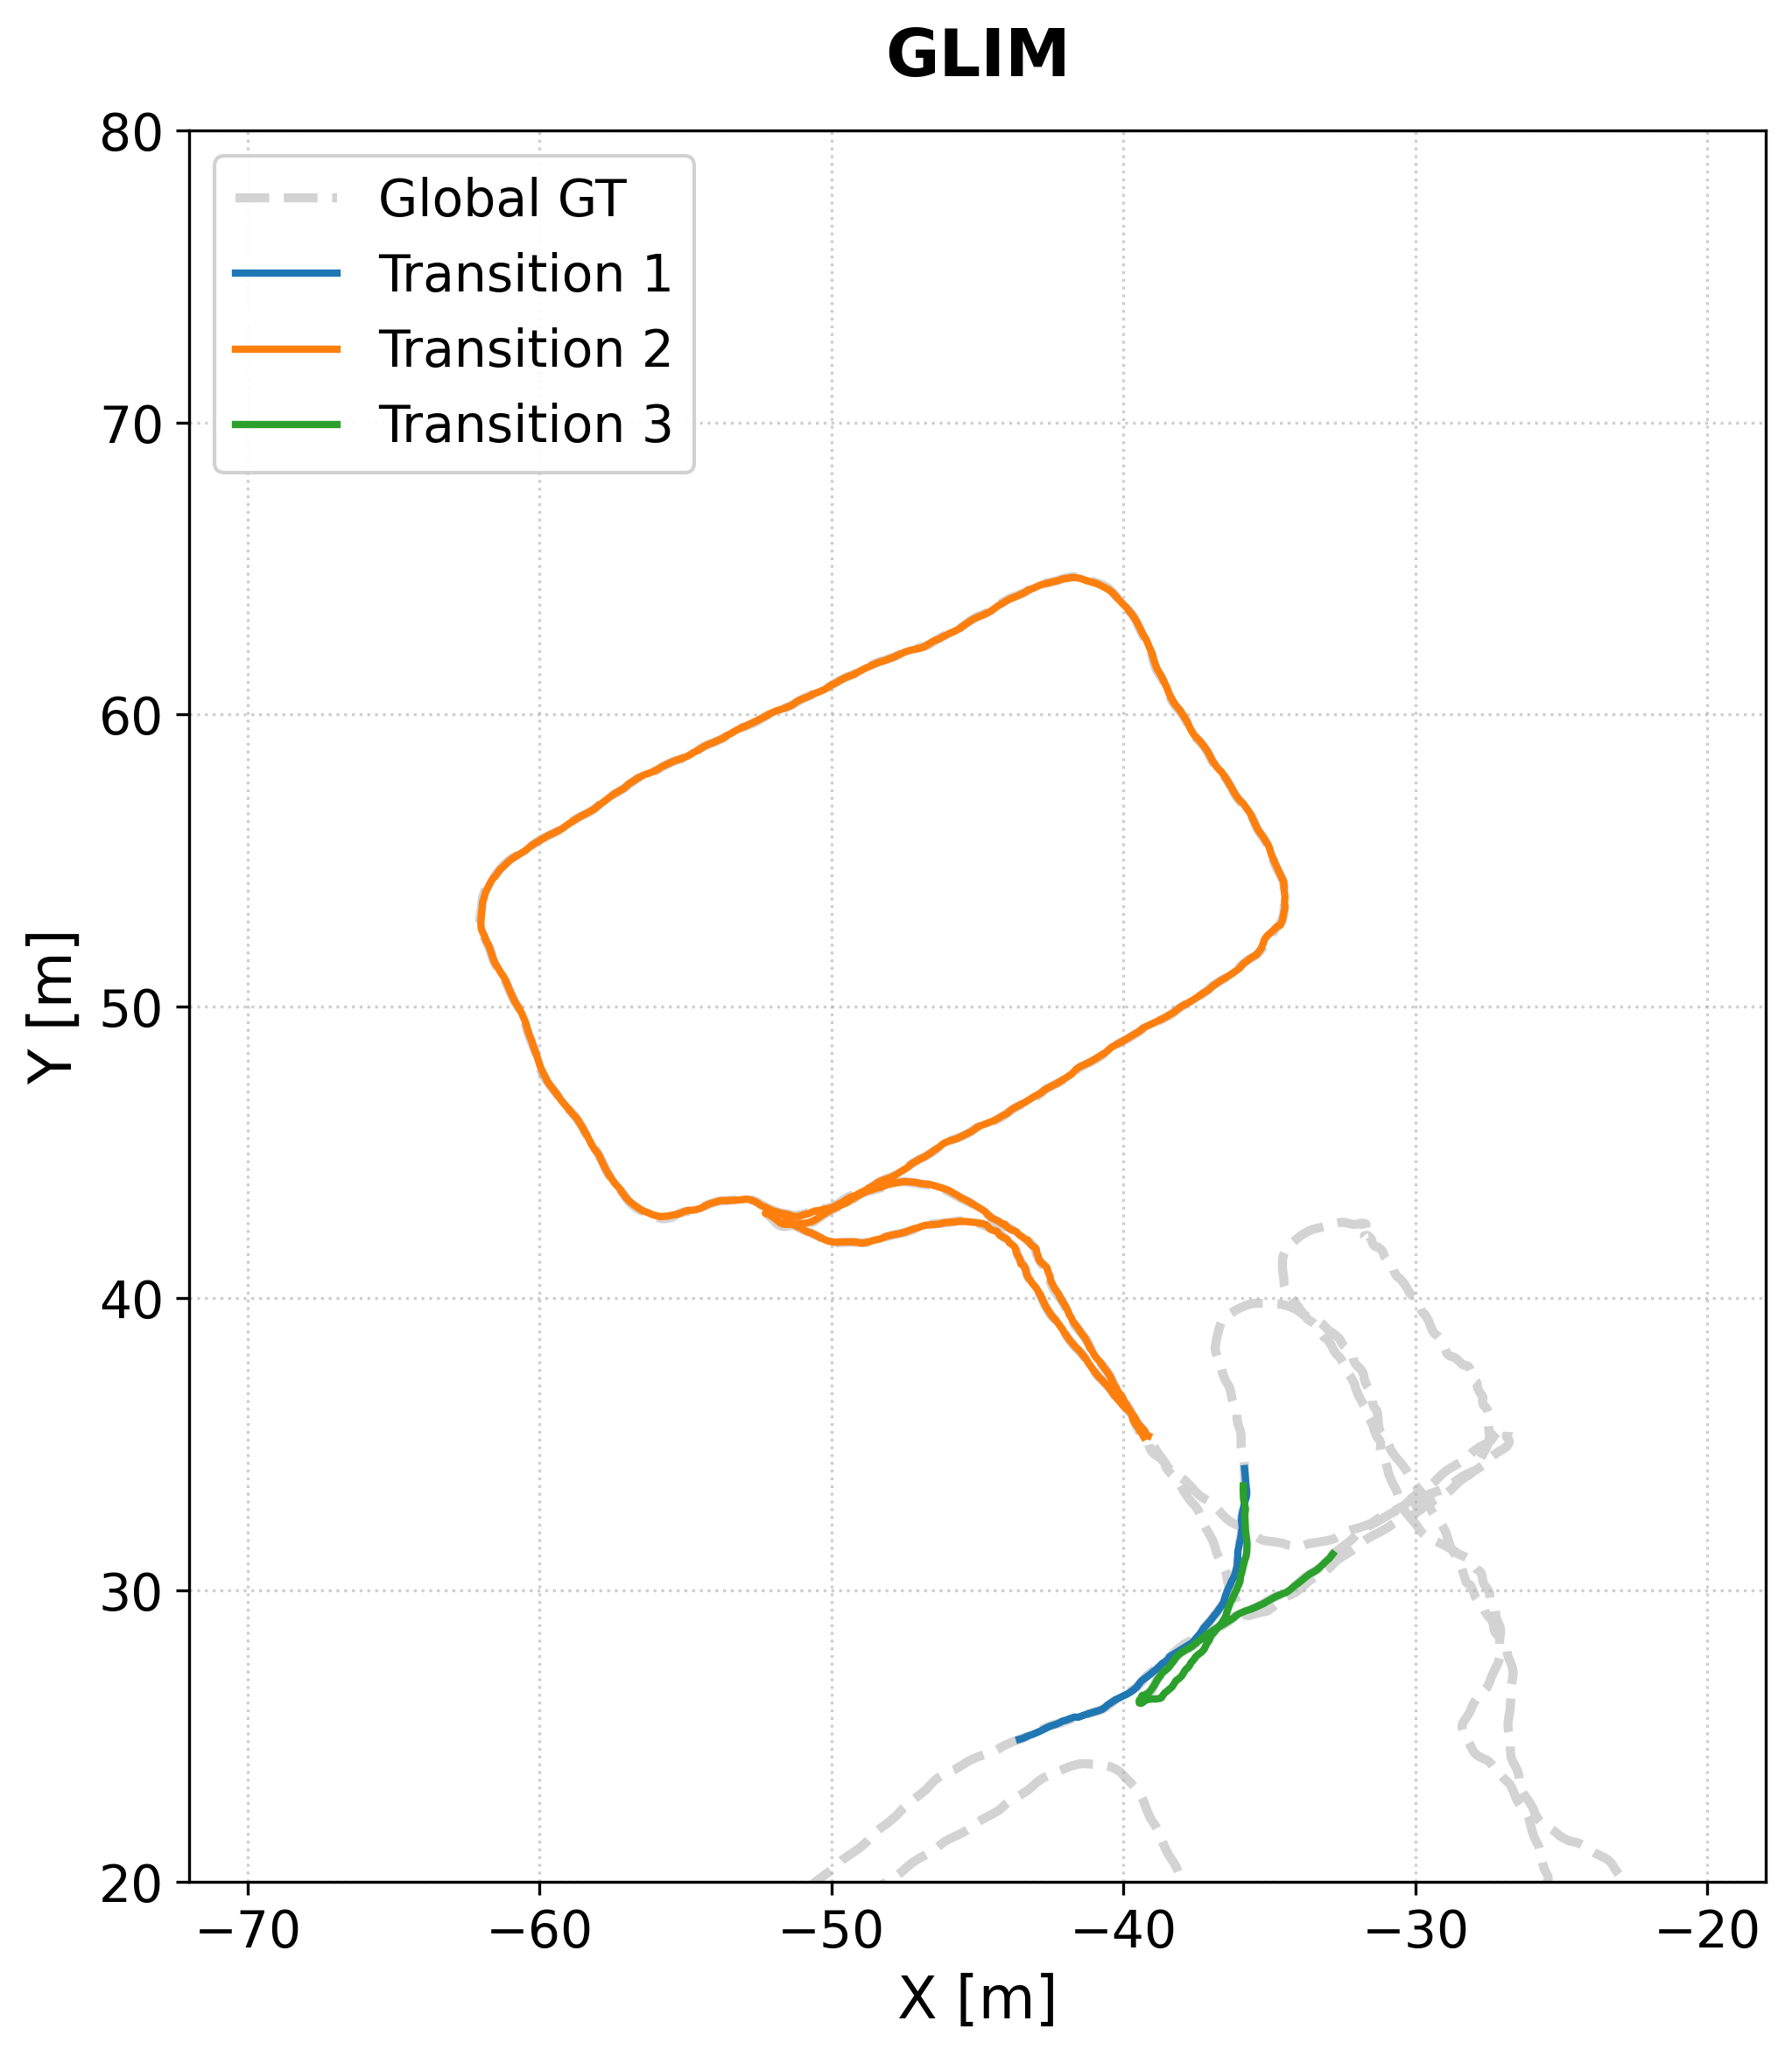
\includegraphics[width=\textwidth]{fig/doorway_transitions_zoom_christ-church-02_glim}
    \end{subfigure}\hfill
    \begin{subfigure}[b]{0.47\textwidth}
        \centering
        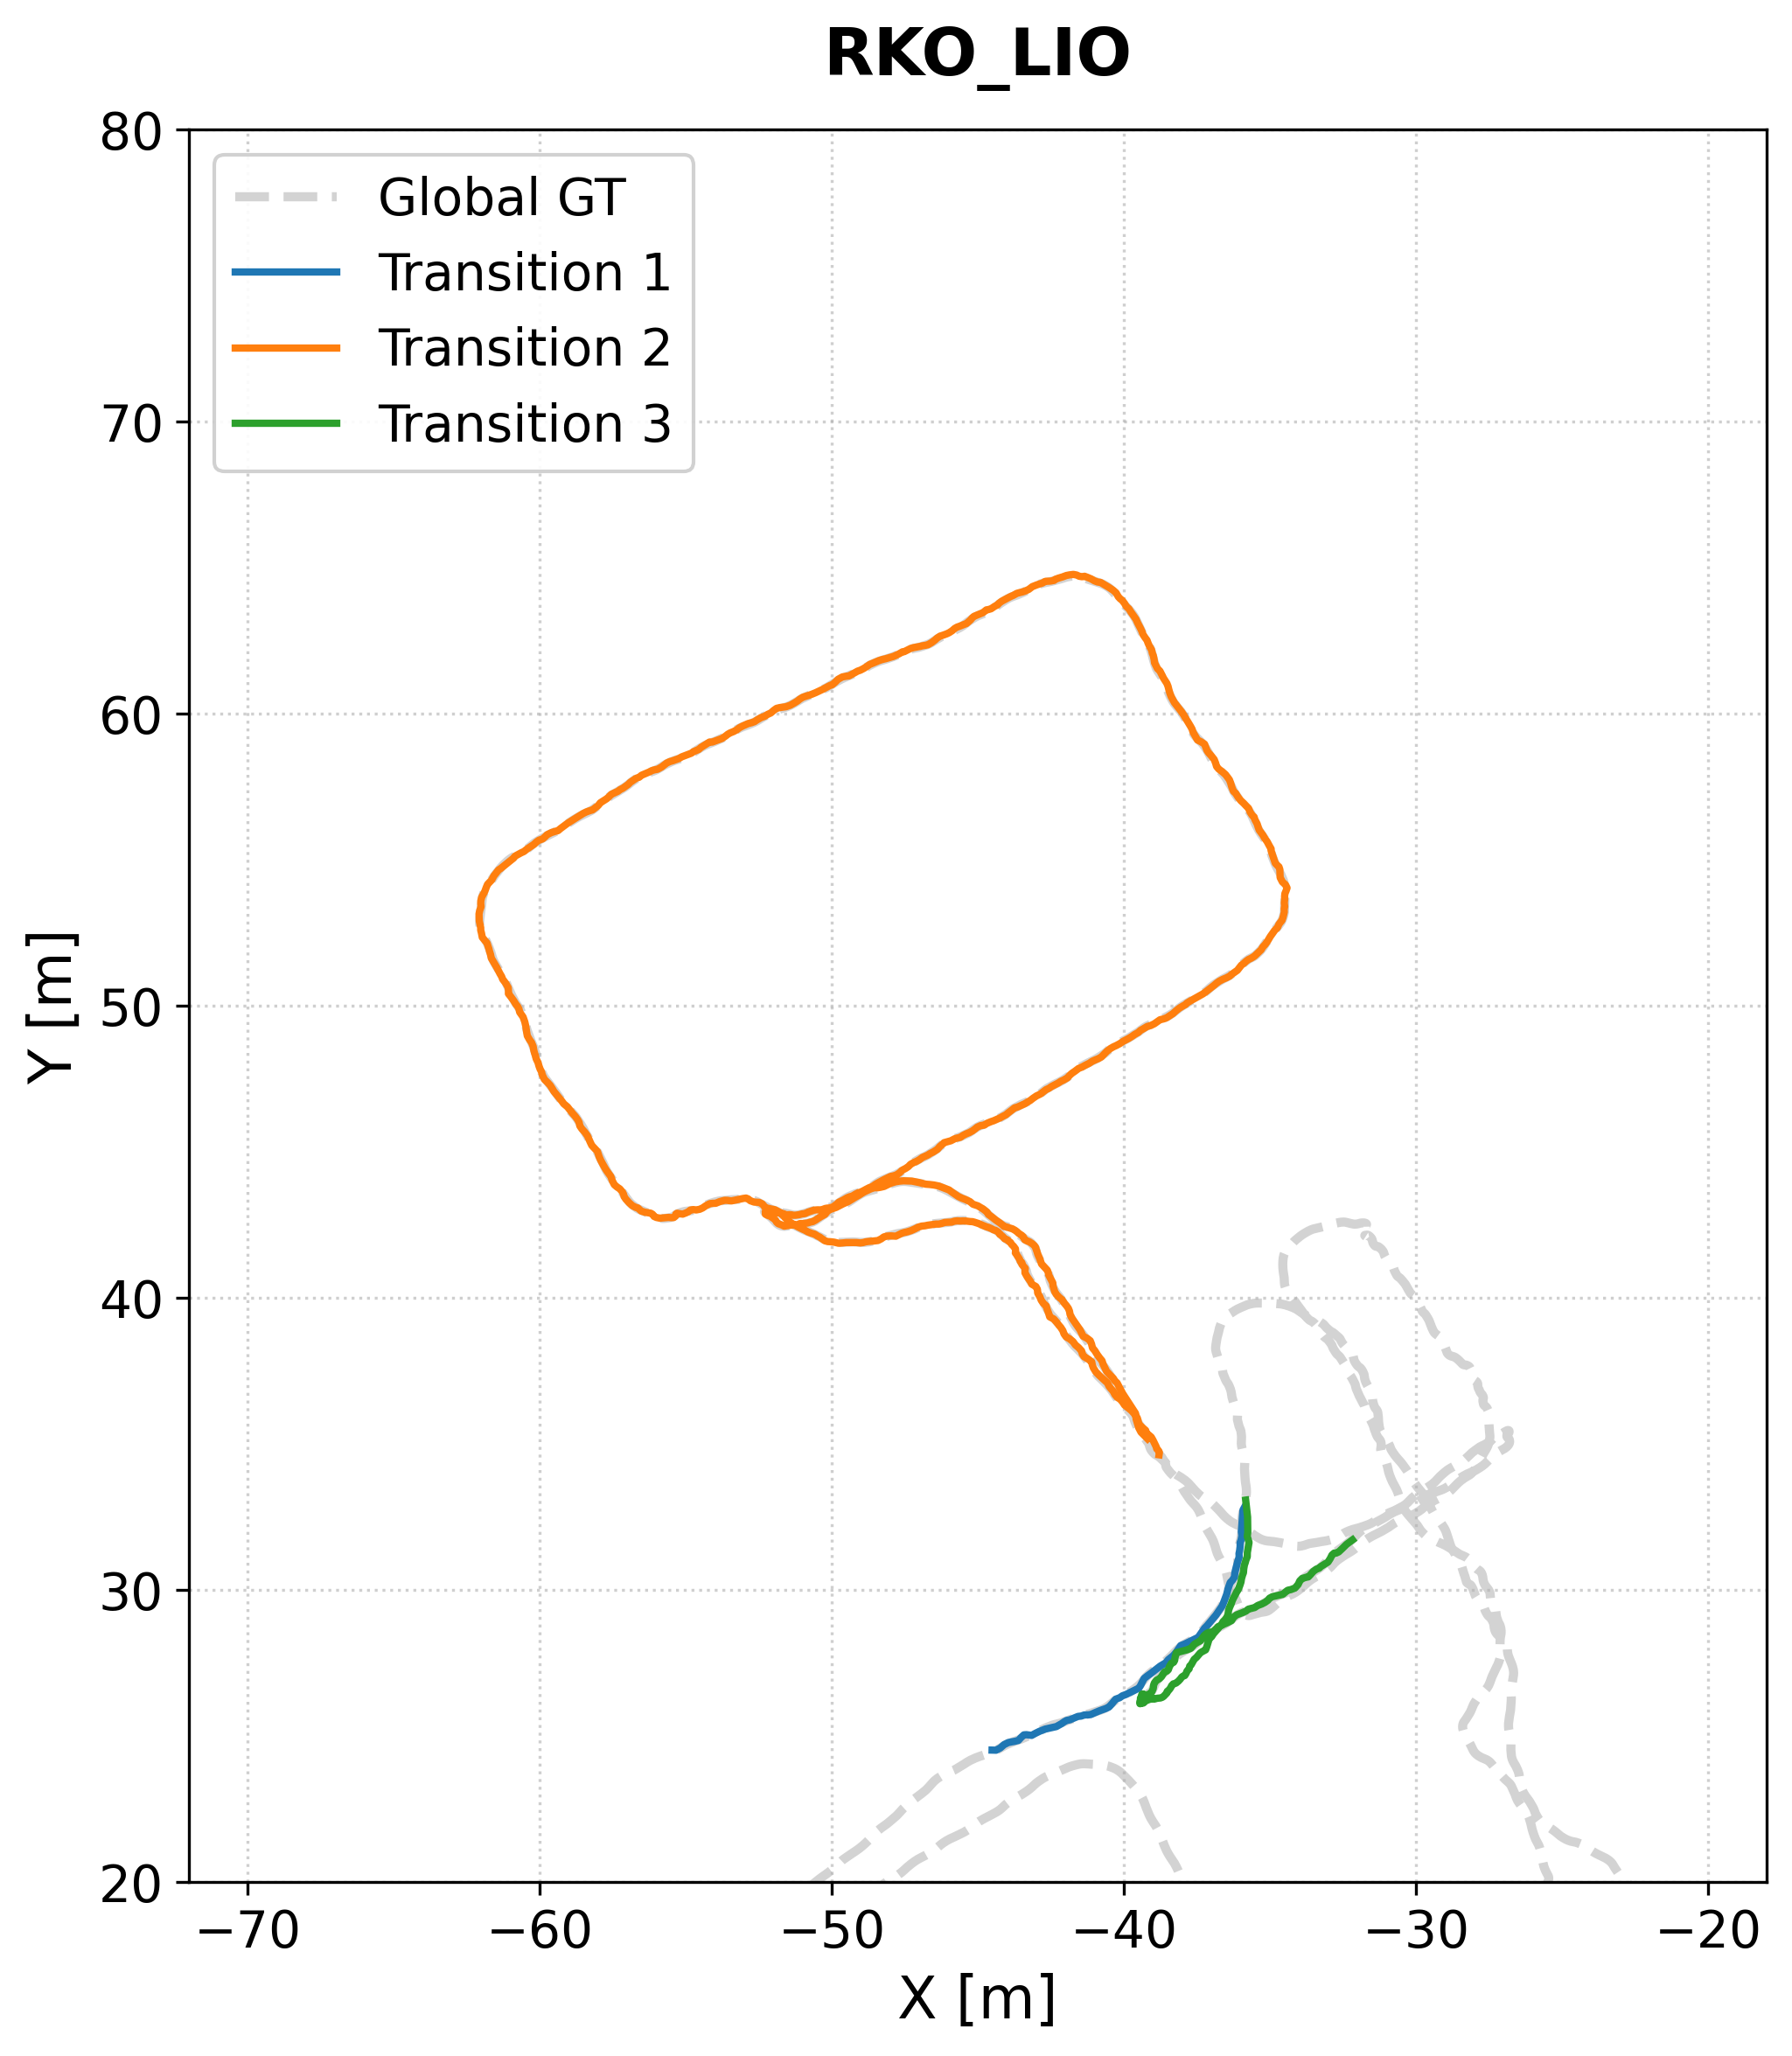
\includegraphics[width=\textwidth]{fig/doorway_transitions_zoom_christ-church-02_rko_lio}
    \end{subfigure}\hfill
    \begin{subfigure}[b]{0.47\textwidth}
        \centering
        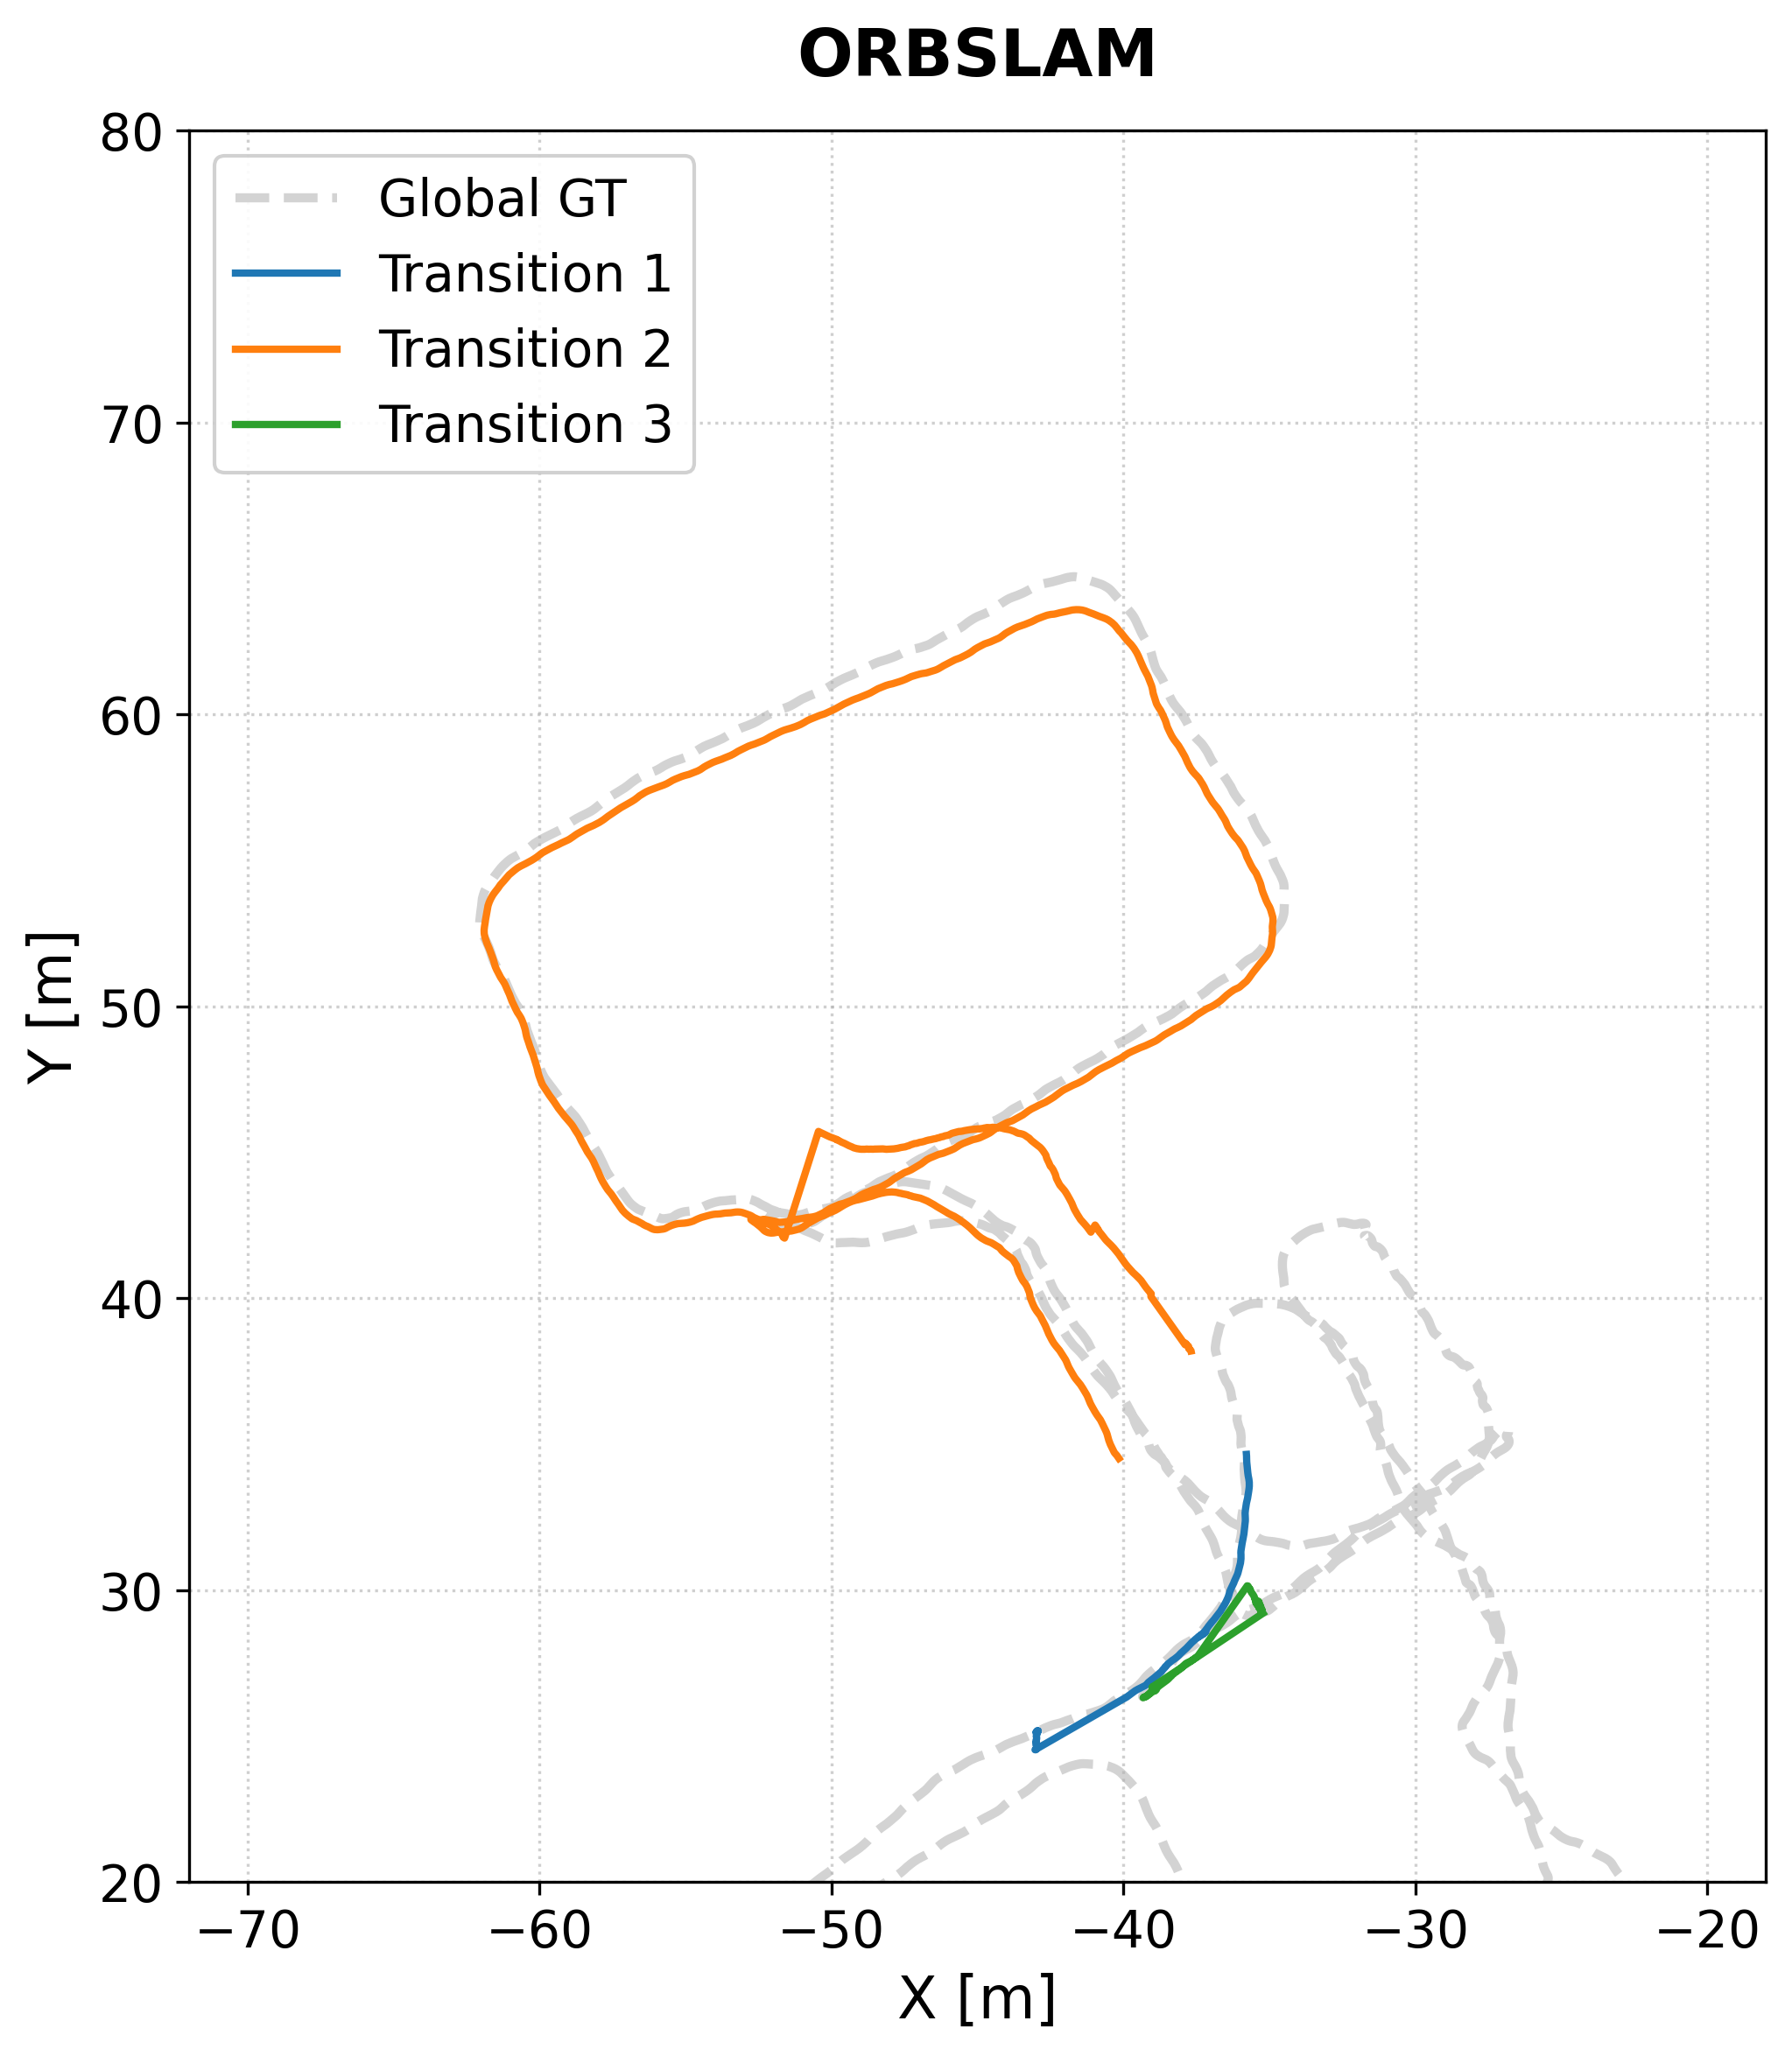
\includegraphics[width=\textwidth]{fig/doorway_transitions_zoom_christ-church-02_orbslam}
    \end{subfigure}\hfill
    \begin{subfigure}[b]{0.47\textwidth}
        \centering
        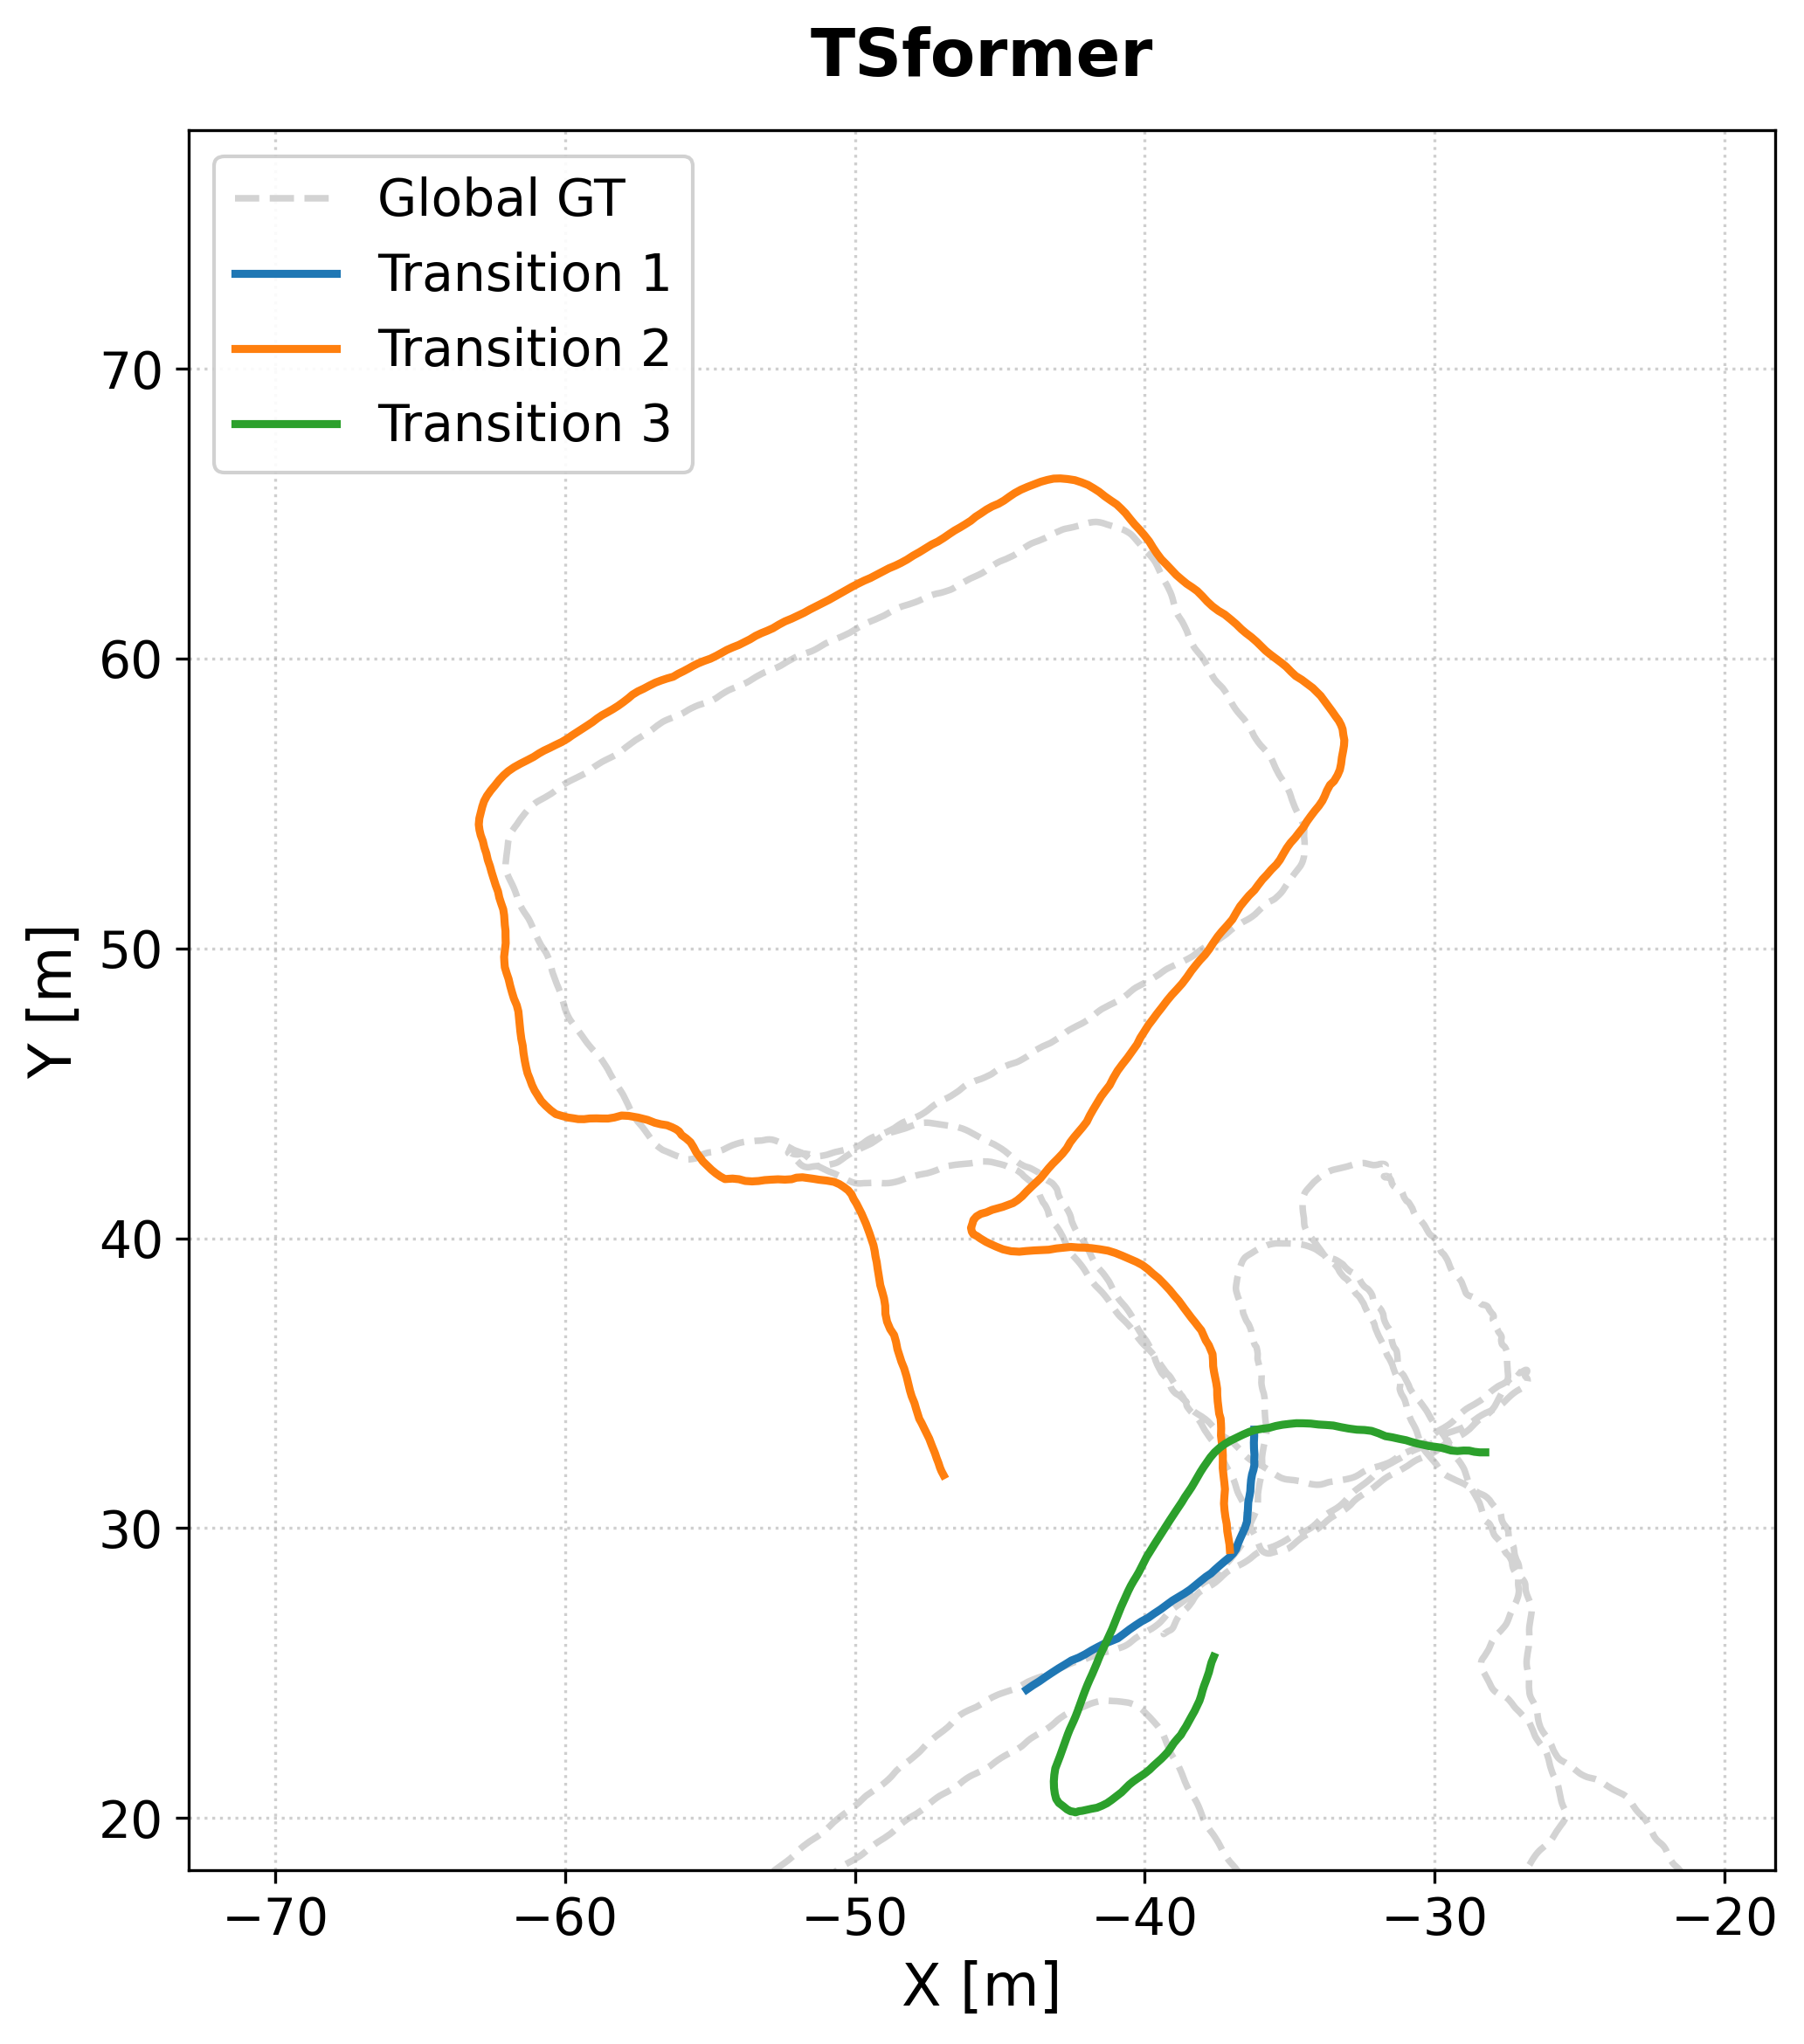
\includegraphics[width=\textwidth]{fig/doorway_transitions_zoom_christ-church-02_tsformer}
    \end{subfigure}

    \caption{Trajectory results for GLIM, RKO\_LIO, ORB-SLAM3 and TSformer plotted during the Transition (Indoor-Outdoor) phases for Seq 02.}
    \label{fig:trajectory_transitions_christ-church-02}
    \vspace{1em} % Vertical space between rows
\end{figure*}


\begin{figure*}
    \centering
    % --- Second Row: christ-church-05 ---
    \begin{subfigure}[b]{0.47\textwidth}
        \centering
        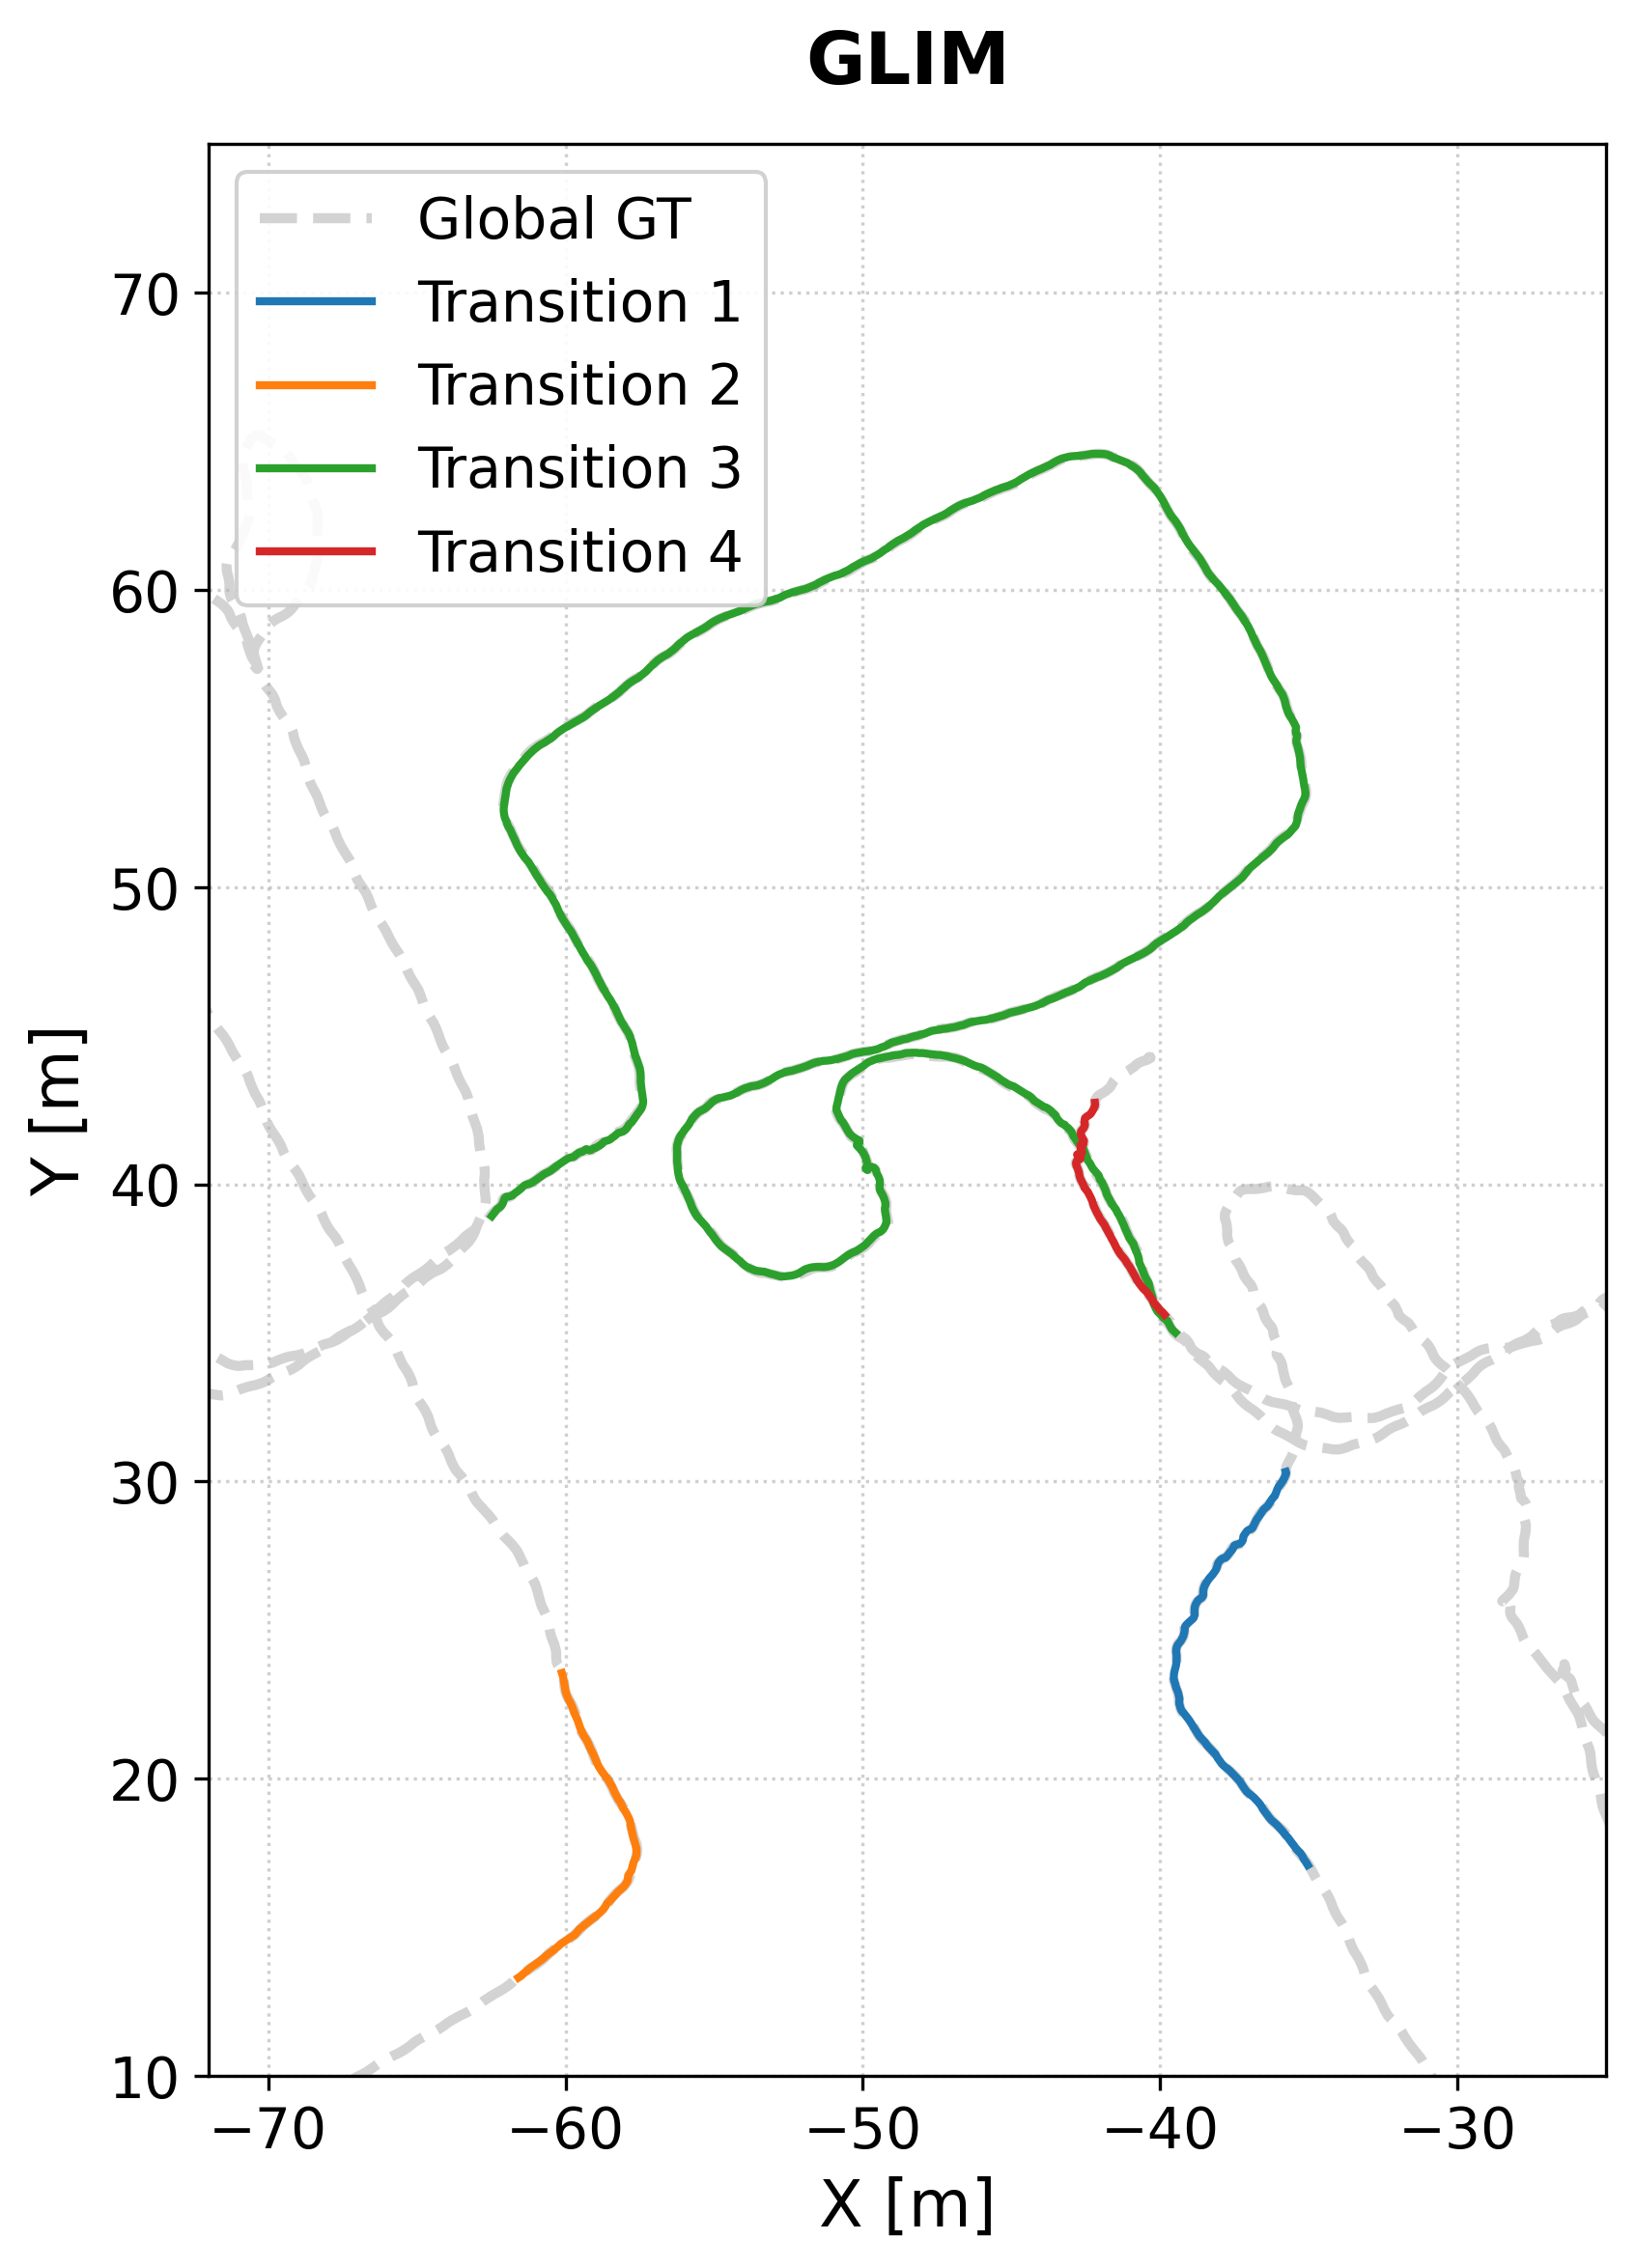
\includegraphics[width=\textwidth]{fig/doorway_transitions_zoom_christ-church-05_glim}
    \end{subfigure}\hfill
    \begin{subfigure}[b]{0.47\textwidth}
        \centering
        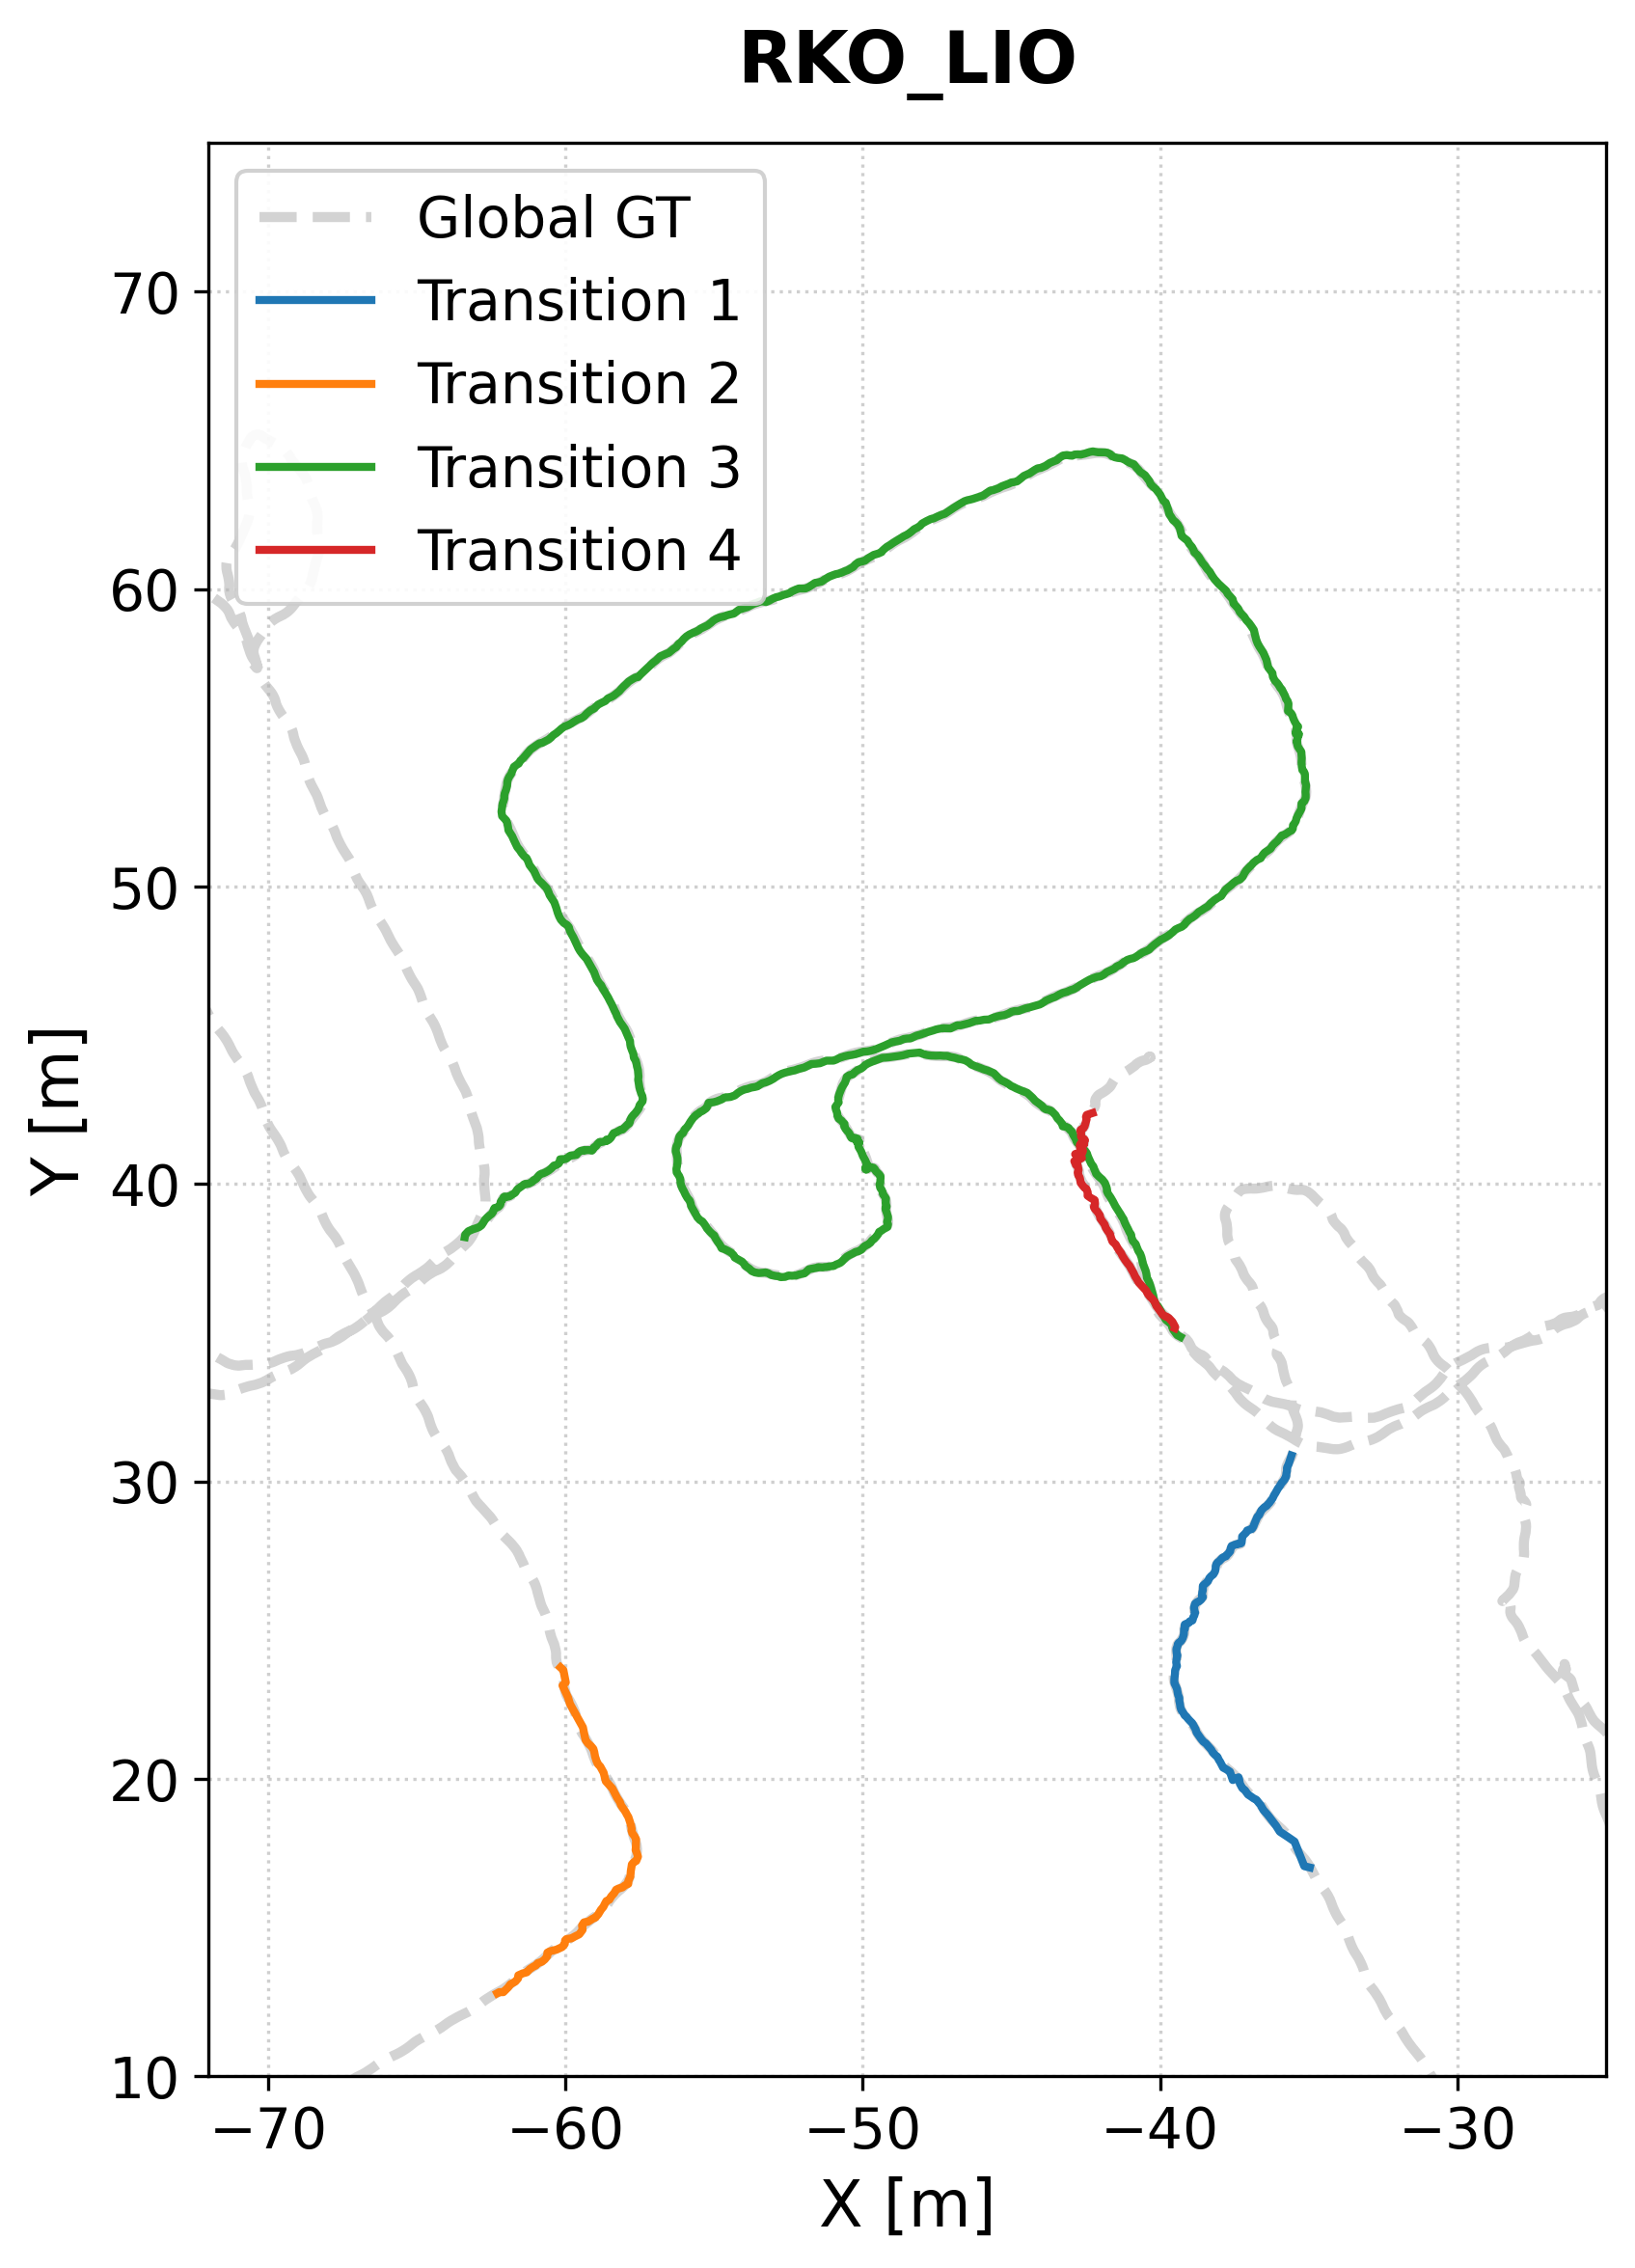
\includegraphics[width=\textwidth]{fig/doorway_transitions_zoom_christ-church-05_rko_lio}
    \end{subfigure}\hfill
    \begin{subfigure}[b]{0.47\textwidth}
        \centering
        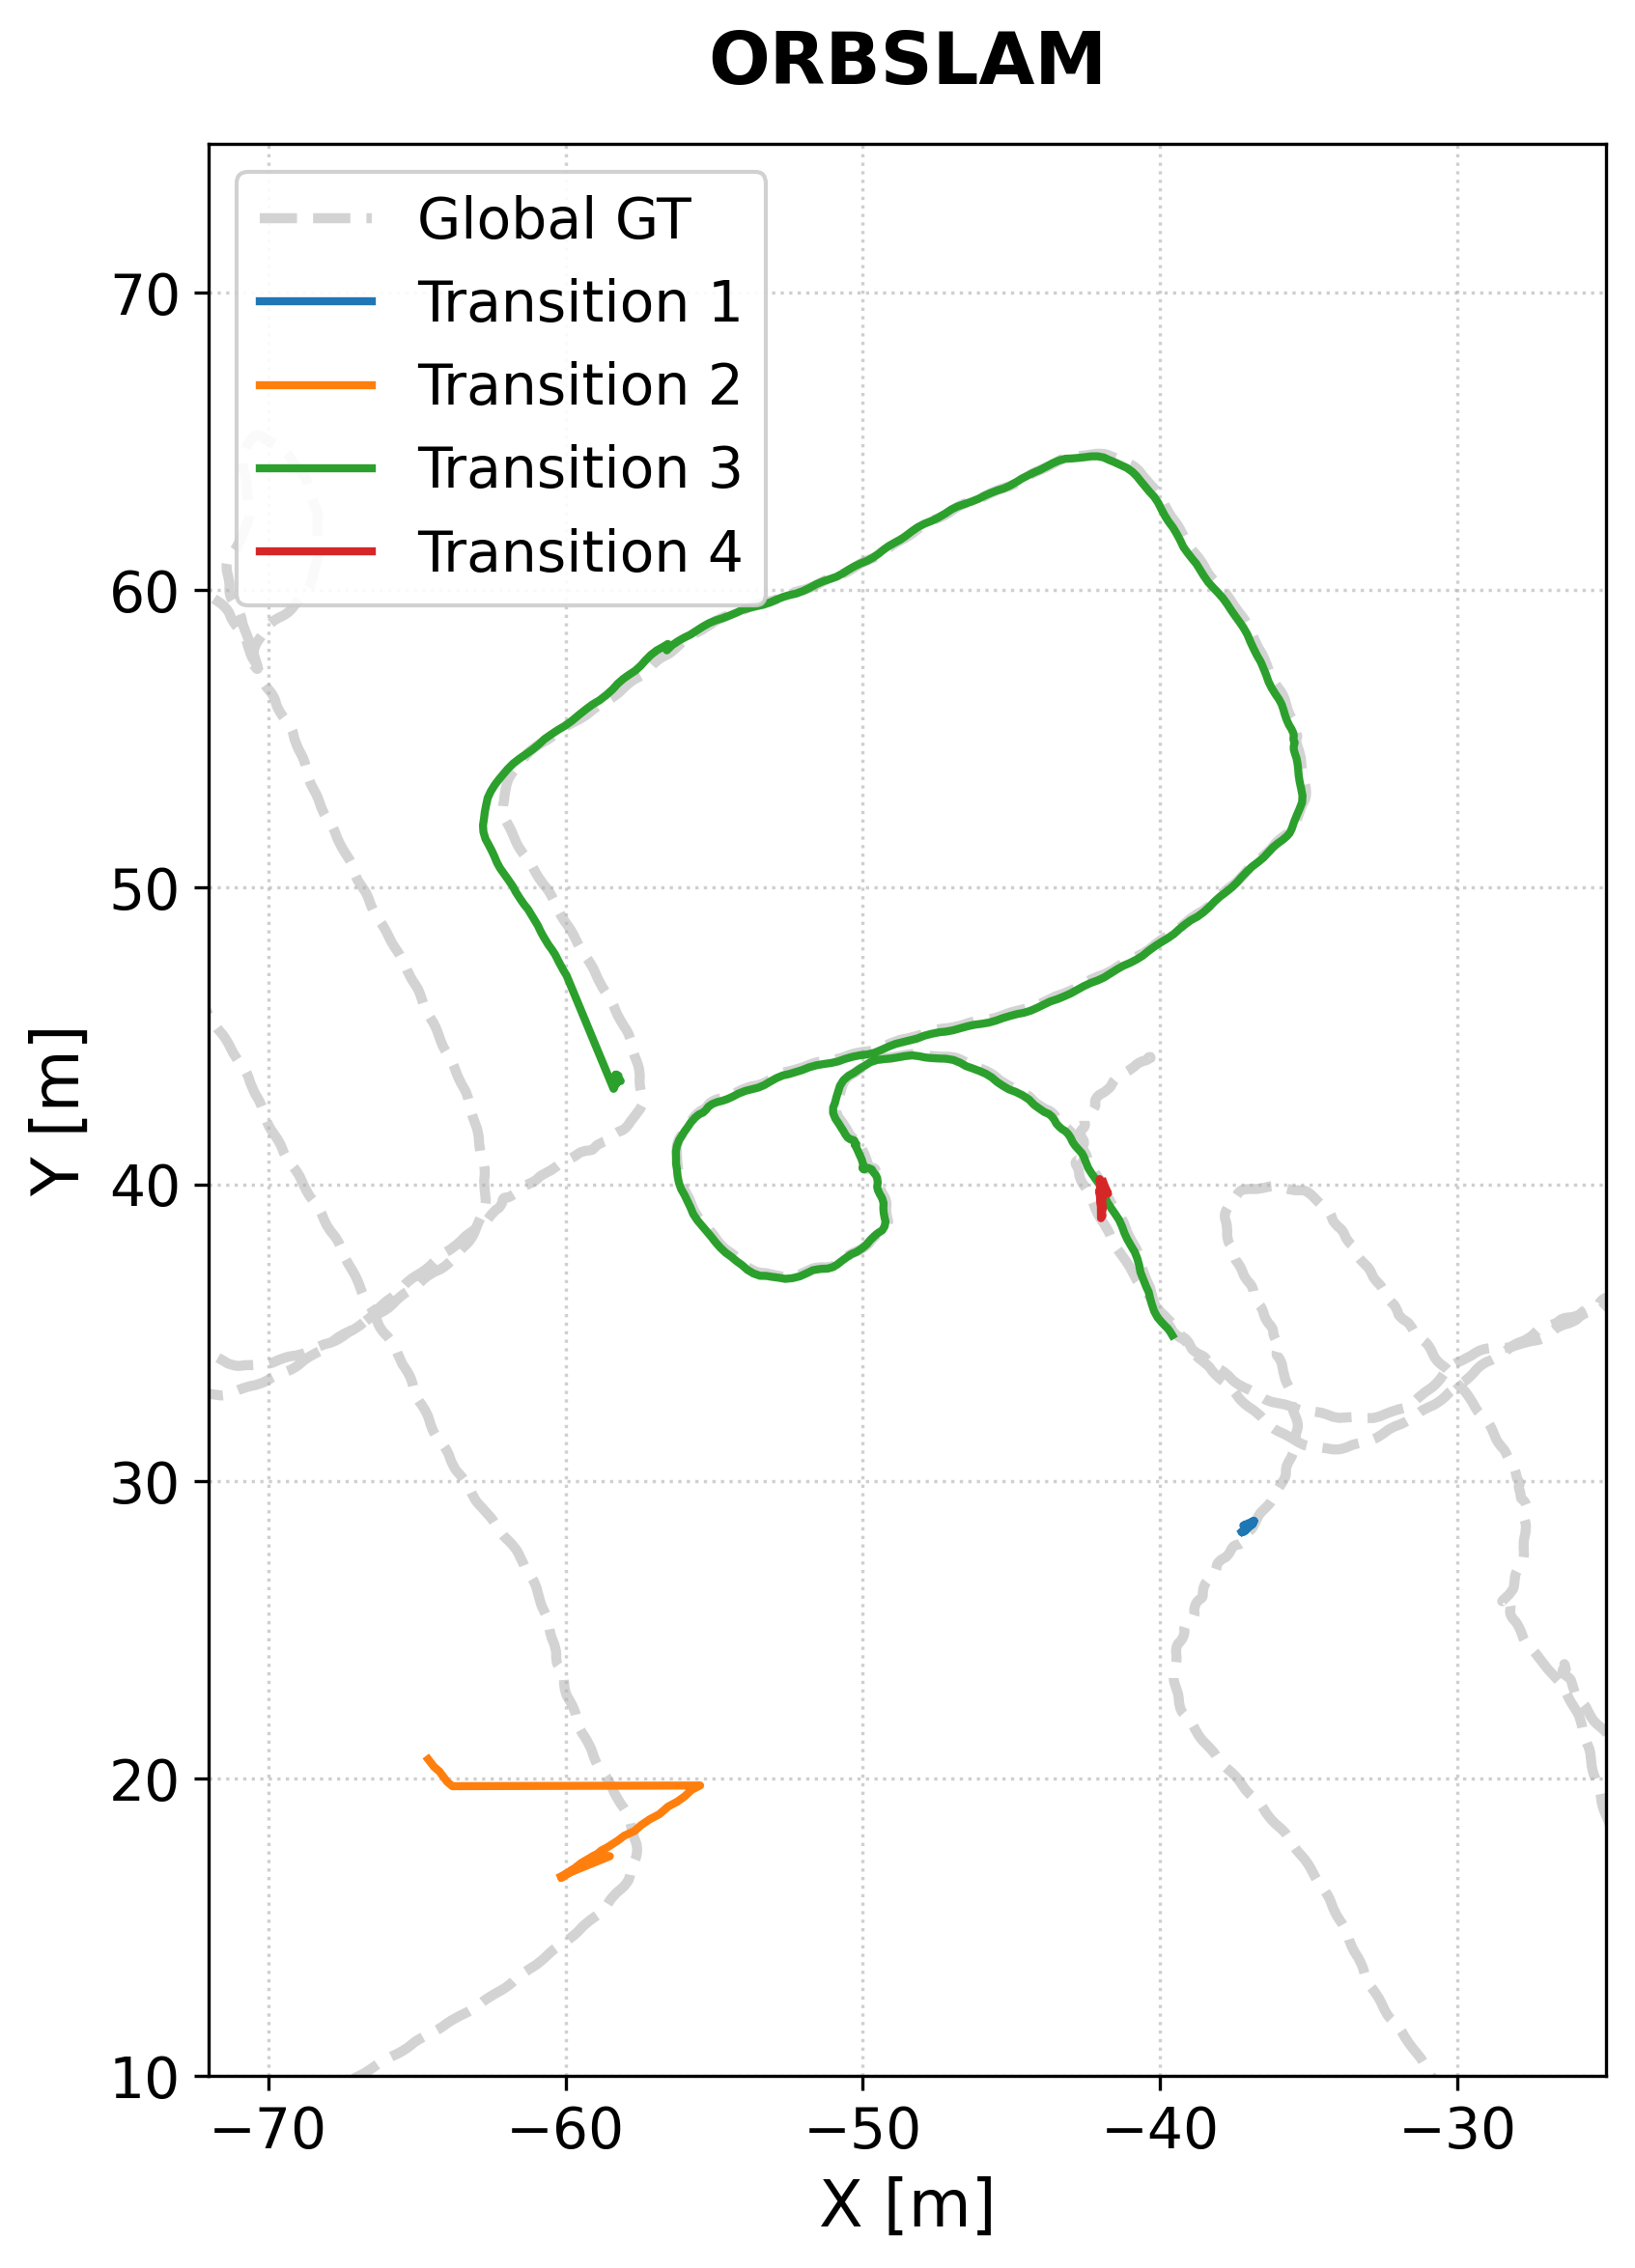
\includegraphics[width=\textwidth]{fig/doorway_transitions_zoom_christ-church-05_orbslam}
    \end{subfigure}\hfill
    \begin{subfigure}[b]{0.47\textwidth}
        \centering
        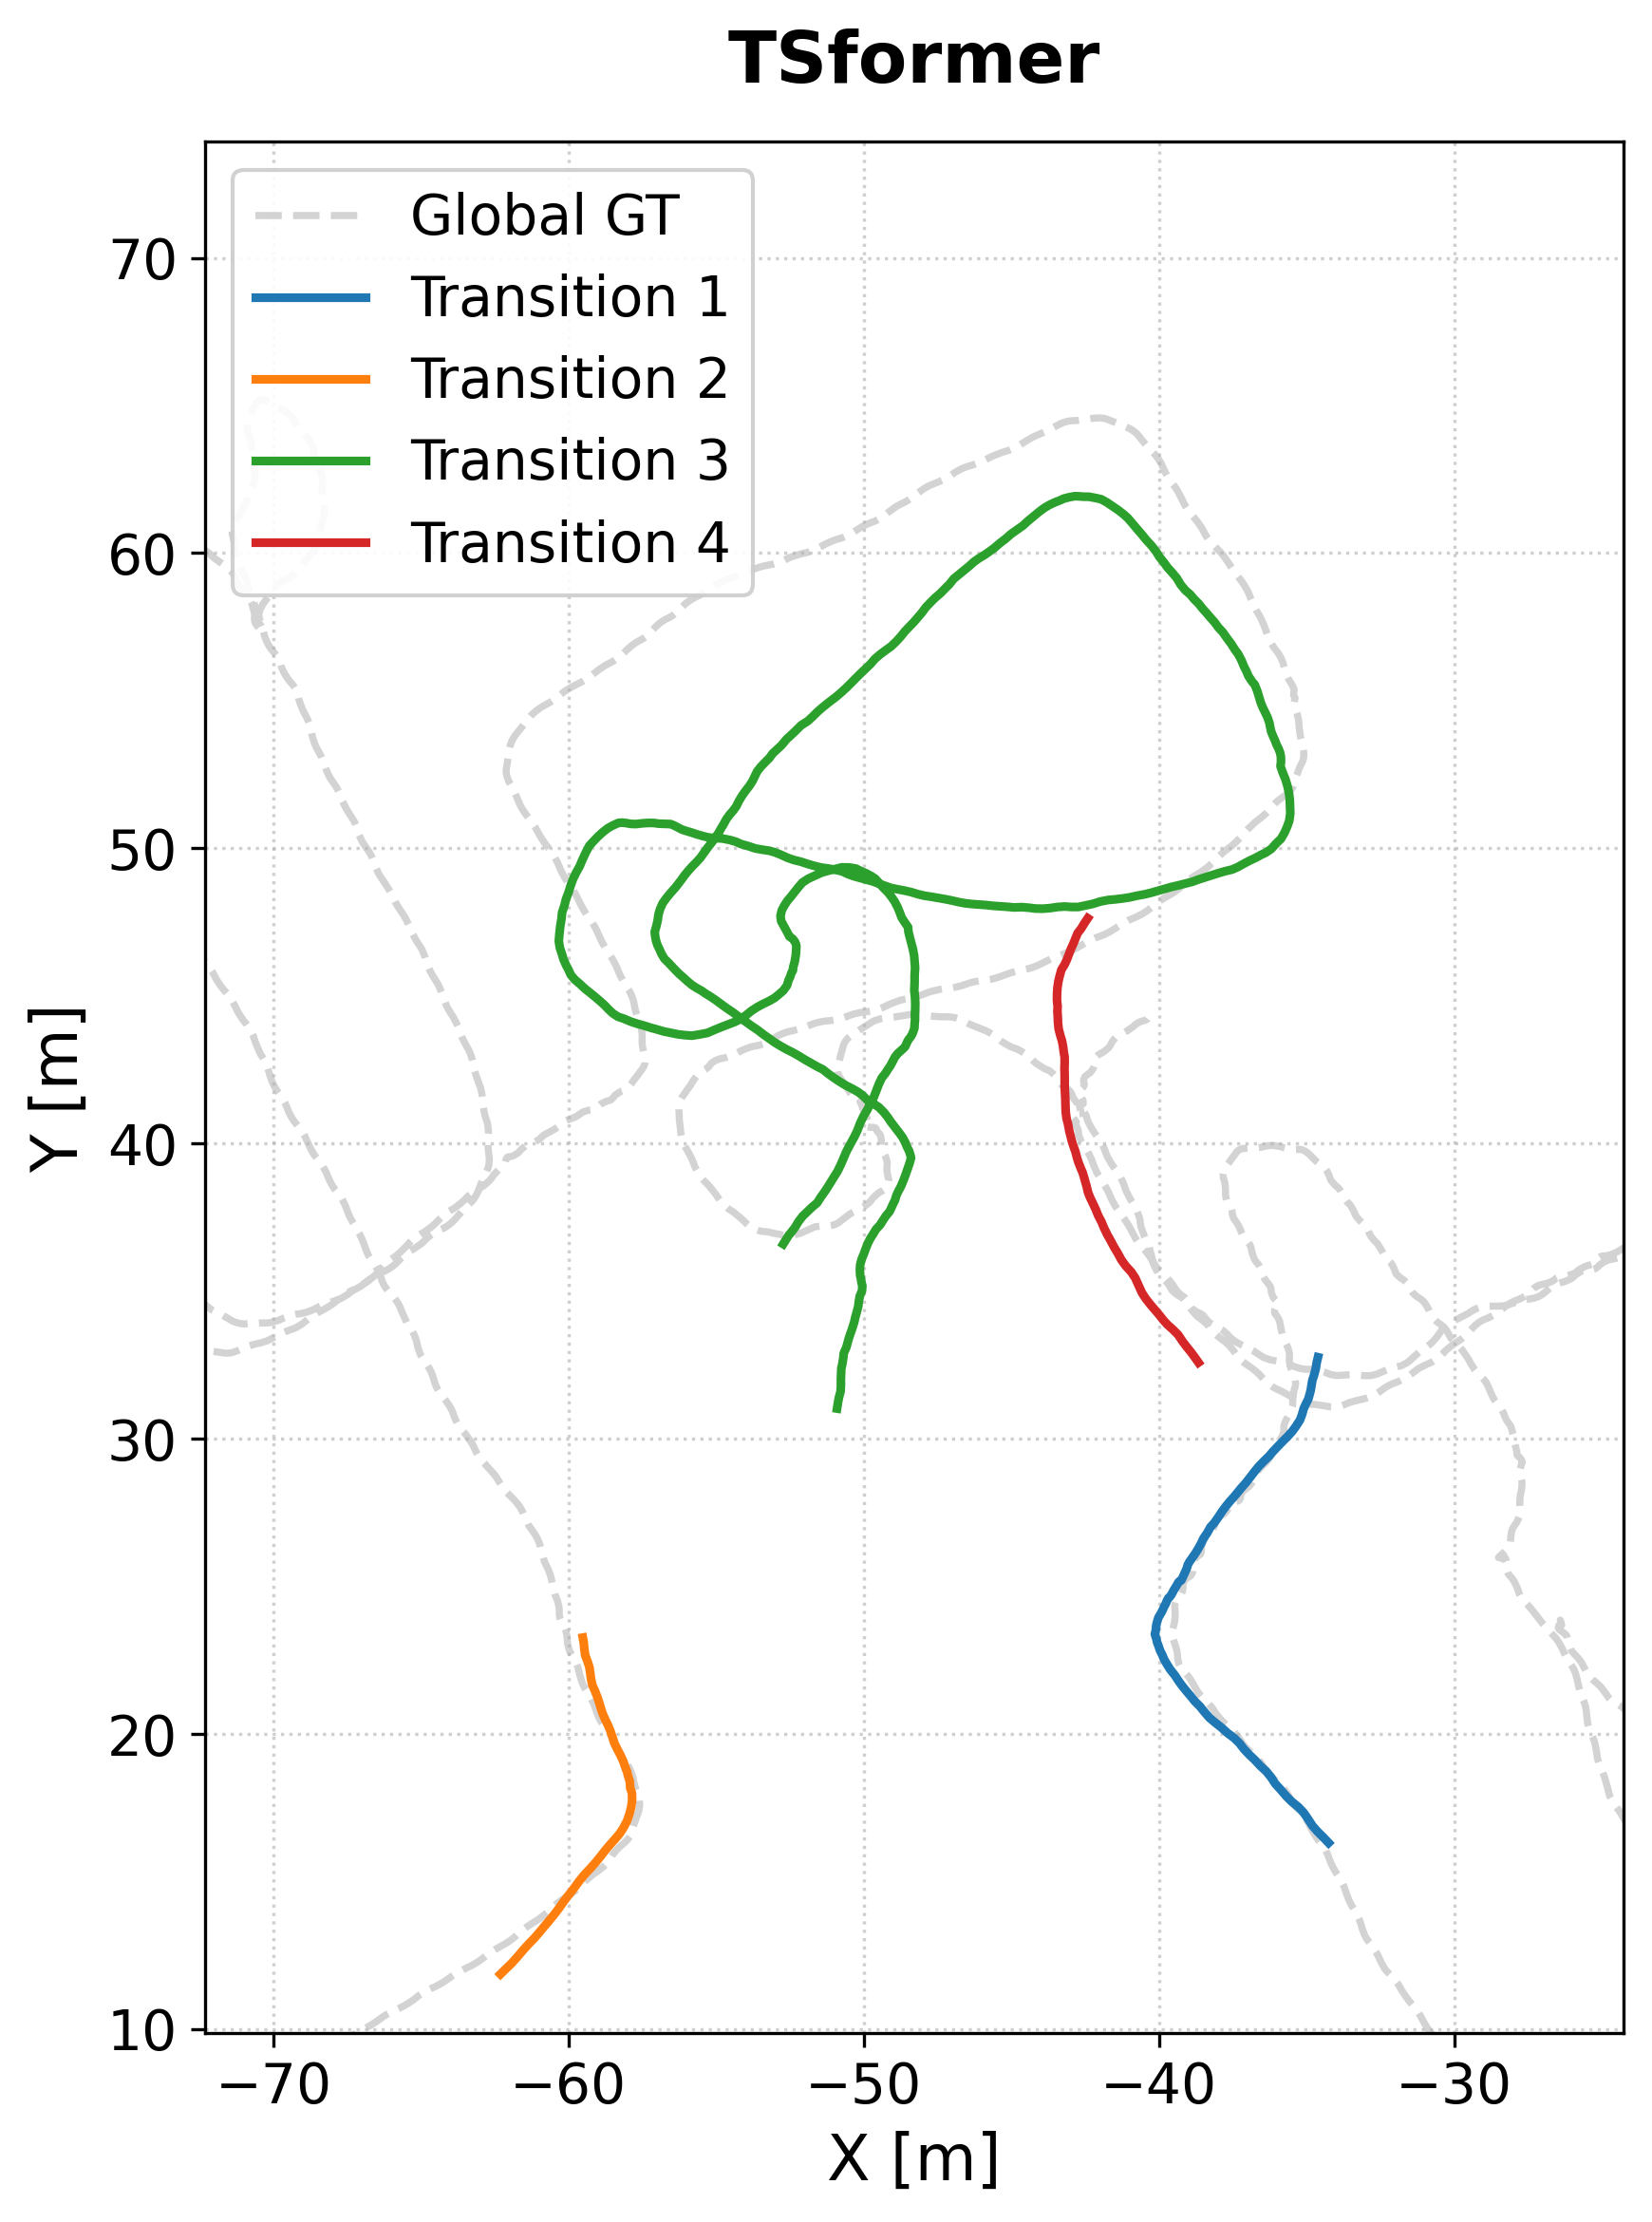
\includegraphics[width=\textwidth]{fig/doorway_transitions_zoom_christ-church-05_tsformer}
    \end{subfigure}
    
    \caption{Trajectory results for GLIM, RKO\_LIO, ORB-SLAM3 and TSformer plotted during the Transition (Indoor-Outdoor) phases for Seq 05.}
    \label{fig:trajectory_transitions_christ-church-05}
\end{figure*}


% \begin{figure*}
% \begin{subfigure}{\textwidth}
%   \centering
%   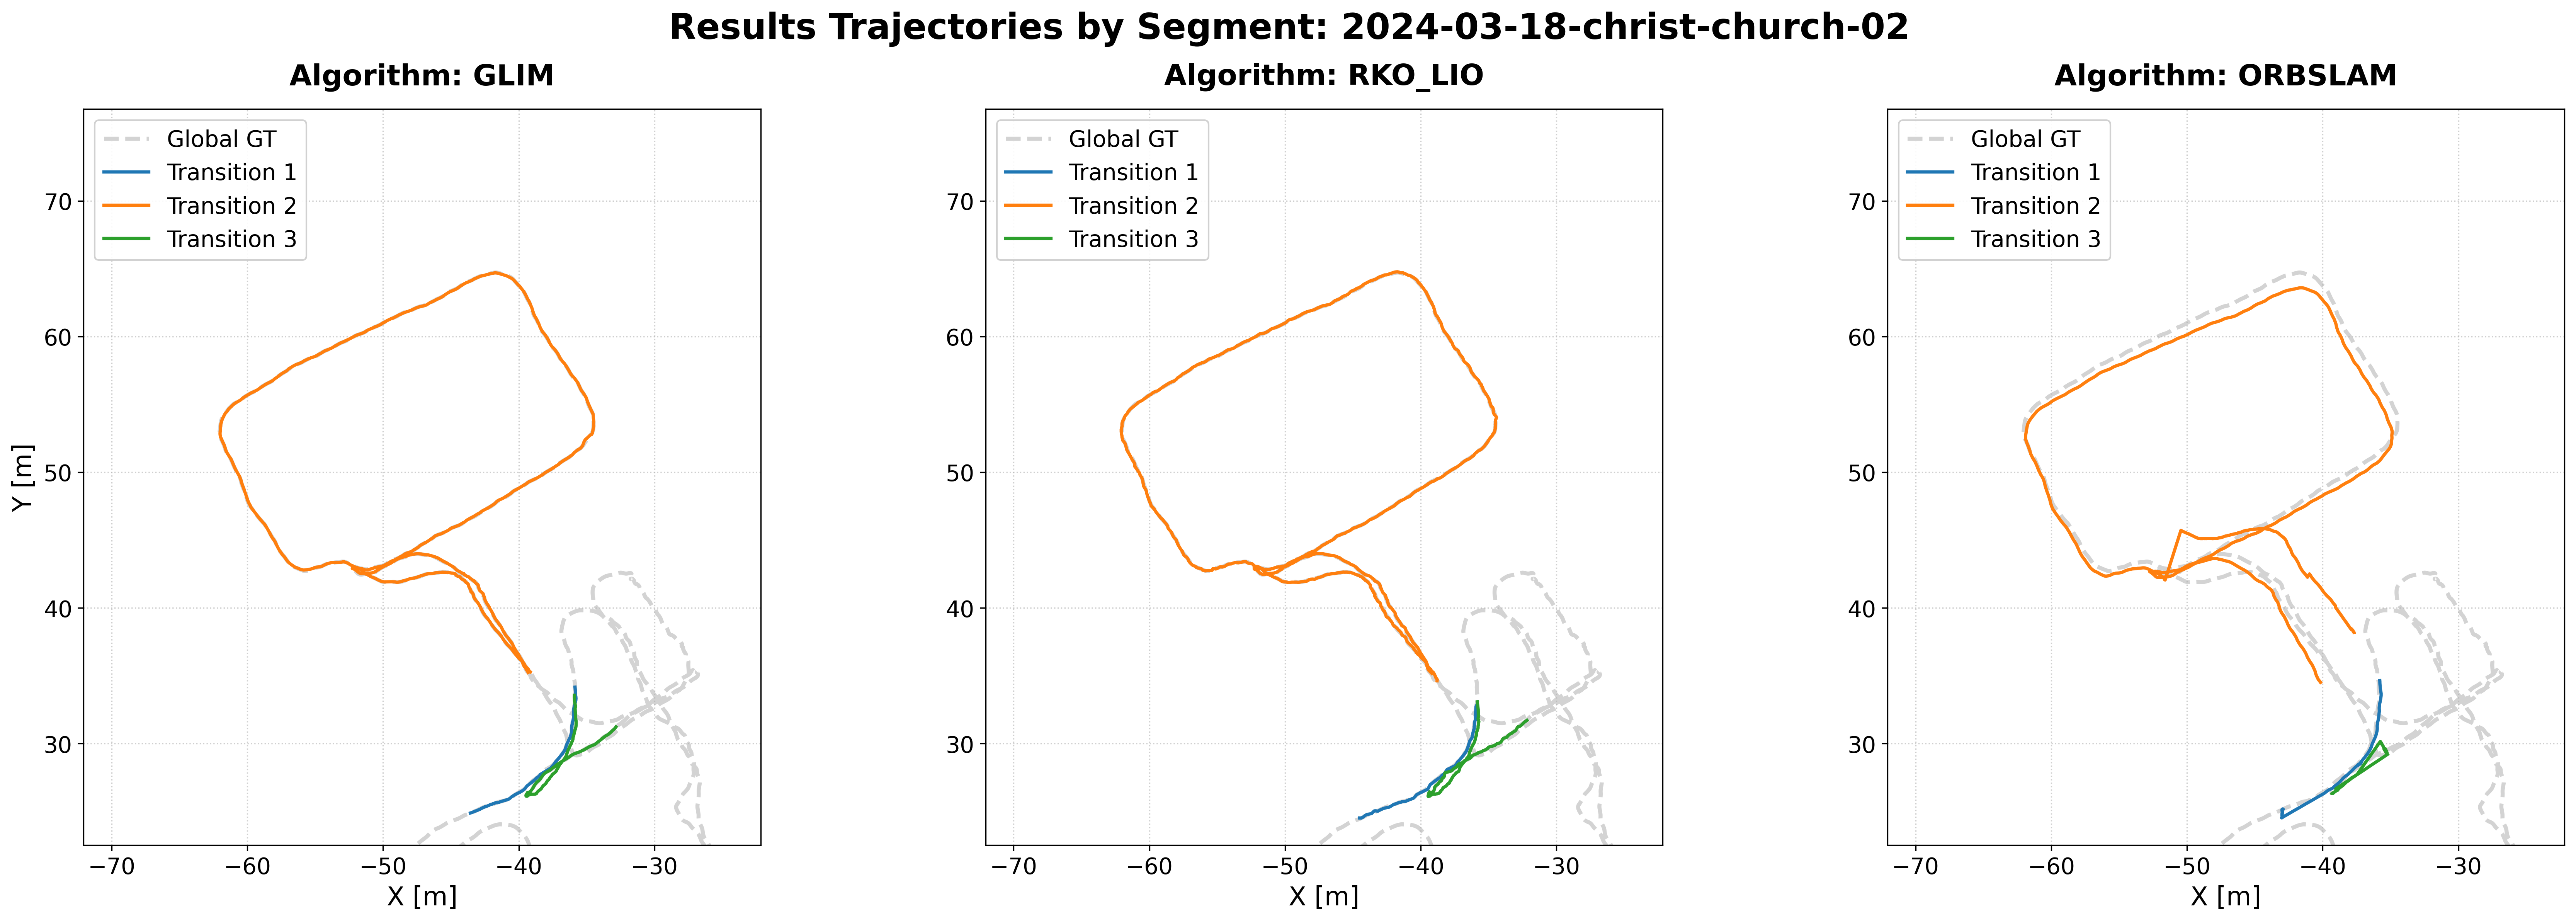
\includegraphics[width=\linewidth]{fig/doorway_transitions_zoom_christ-church-02.png}
%   \label{fig:doorway_transitions_zoom_christ-church-02}
% \end{subfigure}
%     \hfill%
% \begin{subfigure}{\textwidth}
%   \centering
%   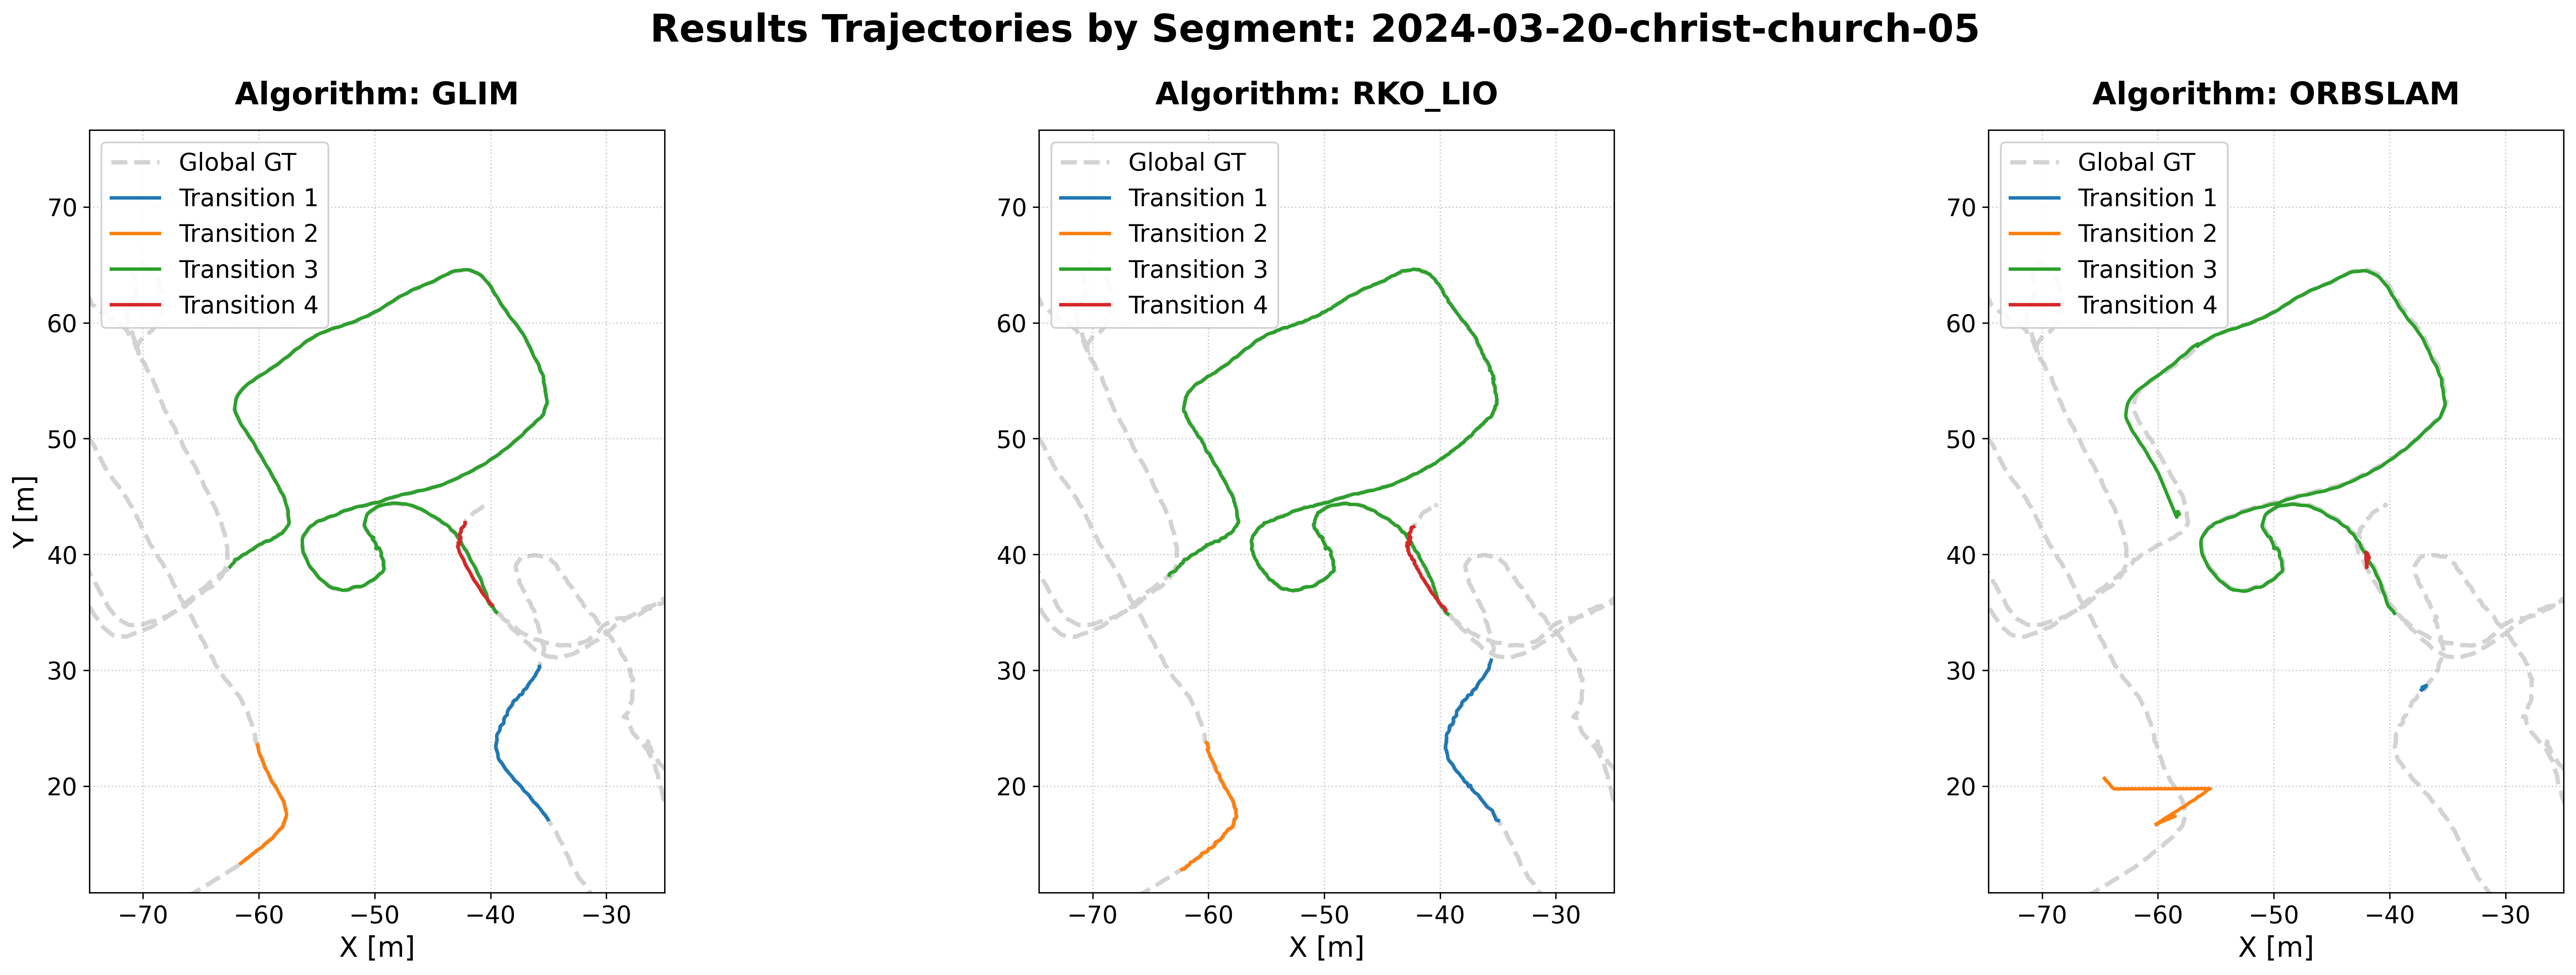
\includegraphics[width=\linewidth]{fig/doorway_transitions_zoom_christ-church-05.png}
%   \label{fig:doorway_transitions_zoom_christ-church-05}
% \end{subfigure}
% \caption{Trajectory results for GLIM, RKO\_LIO, and ORBSLAM plotted during the Transition (Indoor-Outdoor) phases for the tested sequences.}
% \label{fig:trajectory_transitions}
% \end{figure*}


%%%%%%%%%%%%%%%%%%%%%%%%%%%%%%%%%%%%%%%%%%
\section{Conclusions and Future Work}
\label{sec:conclusions}
The research conducted has shown that the greatest challenge for localization systems is not posed by homogeneous working environments, but by transitions between indoor and outdoor environments, where so-called ``stability shocks" occur, caused by the sudden loss or appearance of geometric constraints and rapid changes in lighting conditions. The obtained results empirically confirmed that while state-of-the-art LiDAR-inertial and visual-inertial odometry systems achieve high accuracy in strictly homogeneous environments, their stability is severely challenged during abrupt indoor-outdoor transitions. Optimization-based frameworks with sliding-window historical constraints (e.g. GLIM \cite{Koide_2024}) exhibited the highest resilience against ``stability shocks", whereas vision-dependent systems (e.g. ORB-SLAM3 \cite{ORB-SLAM3}) proved vulnerable to transient exposure anomalies despite maintaining tight local accuracy under stable lighting. The evaluated learning-based TSformer-VO baseline showed competitive local relative motion estimates in several segments, but its larger absolute drift across indoor, outdoor, and transition regimes indicates that improving global consistency currently represents a major barrier to their application.

The vulnerabilities identified in this benchmark directly inform our future research trajectory. To achieve true mixed-environment autonomy, reliance on rigid, single-paradigm state estimators is insufficient. Our future work will focus on the following key directions:
\begin{itemize}
    \item \textbf{Adaptive Multi-Modal Data Fusion:} We plan to develop a tightly-coupled, dynamically weighted sensor fusion algorithm. By monitoring real-time covariance stability and geometric degeneracy metrics (e.g. eigenvalue analysis of the point cloud covariance), the proposed system will adaptively shift trust between visual, LiDAR, and inertial constraints when crossing building thresholds.
    \item \textbf{GNSS/RTK Integration for Global Consistency:} While this study focused on local transition shocks, long-term outdoor navigation necessitates absolute positioning. Future frameworks will incorporate RTK-GNSS factors into the optimization graph, with specific emphasis on handling multi-path effects and signal degradation at the urban canyon/indoor area.
    \item \textbf{Robustness in Degraded Conditions:} The benchmark will be expanded to include datasets featuring adverse weather (rain, fog) and low-light scenarios, which commonly affect industrial mobile robots. This will test the limits of LiDAR intensity returns and sensor-agnostic modeling in maintaining odometry continuity.
\end{itemize}
The conclusions from the conducted research will serve as the basis for the development of a novel, comprehensive localization system for mobile industrial robots, designed to maintain robust localization performance under the abrupt changes in perception conditions associated with transitions between indoor and outdoor environments.

\backmatter

% \bmhead{Supplementary information}

% If your article has accompanying supplementary file/s please state so here.

% Authors reporting data from electrophoretic gels and blots should supply the full unprocessed scans for key as part of their Supplementary information. This may be requested by the editorial team/s if it is missing.

% Please refer to Journal-level guidance for any specific requirements.

% \bmhead{Acknowledgments}

% Acknowledgments are not compulsory. Where included they should be brief. Grant or contribution numbers may be acknowledged.

% Please refer to Journal-level guidance for any specific requirements.
\section*{Declarations}

\subsection*{Funding}
This research received no external funding.

\subsection*{Conflicts of interest/Competing interests}
The authors have no conflicts of interest to declare that are relevant to the content of this article.

\subsection*{Data Availability}
The Oxford Spires Dataset used in this study is publicly available at \url{https://dynamic.robots.ox.ac.uk/datasets/oxford-spires/} and is described in the associated data paper available at \url{https://doi.org/10.1177/02783649251369905}. The dataset is distributed under the Creative Commons Attribution-NonCommercial-ShareAlike 4.0 International (CC BY-NC-SA 4.0) license. The trajectory segmentations generated and analysed during the current study are available from the corresponding author, Piotr Duszak (\href{mailto:piotr.duszak@pw.edu.pl}{piotr.duszak@pw.edu.pl}), upon reasonable request.

The original pretrained weights for the TSformer-VO model are publicly available at \url{https://github.com/aofrancani/TSformer-VO} under the MIT License. The publication describing the model is available at \url{https://doi.org/10.1109/ACCESS.2025.3531667}. The TSformer-VO weights fine-tuned during the current study are available from the corresponding author, Piotr Duszak (\href{mailto:piotr.duszak@pw.edu.pl}{piotr.duszak@pw.edu.pl}), upon reasonable request.


\subsection*{Code Availability}
The code is available at github repository at \url{https://github.com/Cassie051/localization-benchamark}.



\subsection*{Authors' Contributions}

\textbf{K.K.} methodology, software, formal analysis, investigation, resources, data curation, writing - original draft preparation.

\noindent
\textbf{J.D.} conceptualization, supervision, project administration, funding acquisition, writing - review and editing.

\noindent
\textbf{P.D.} conceptualization, methodology, validation, resources, writing - original draft preparation, writing - review and editing.


\subsection*{Acknowledgments}
The authors acknowledge the support of the High Performance Computing Center at the Faculty of Mathematics and Information Science, Warsaw University of Technology, which provided computational resources for this research.

\subsection*{Ethics approval}
Not applicable

\subsection*{Consent to participate}
Not applicable

\subsection*{Consent for publication}
Not applicable

\bibliography{sn-bibliography}% common bib file
%% if required, the content of .bbl file can be included here once bbl is generated
%%\input sn-article.bbl


\end{document}
